% Options for packages loaded elsewhere
\PassOptionsToPackage{unicode}{hyperref}
\PassOptionsToPackage{hyphens}{url}
\PassOptionsToPackage{dvipsnames,svgnames,x11names}{xcolor}
%
\documentclass[
  10pt,
  a4paper,
]{article}
\usepackage{amsmath,amssymb}
\usepackage{iftex}
\ifPDFTeX
  \usepackage[T1]{fontenc}
  \usepackage[utf8]{inputenc}
  \usepackage{textcomp} % provide euro and other symbols
\else % if luatex or xetex
  \usepackage{unicode-math} % this also loads fontspec
  \defaultfontfeatures{Scale=MatchLowercase}
  \defaultfontfeatures[\rmfamily]{Ligatures=TeX,Scale=1}
\fi
\ifPDFTeX\else
  % xetex/luatex font selection
  \setmainfont[]{Liberation Serif}
  \setsansfont[]{Liberation Sans}
  \setmonofont[Scale=0.82]{DejaVu Sans Mono}
  \setmathfont[]{DejaVu Math TeX Gyre}
\fi
% Use upquote if available, for straight quotes in verbatim environments
\IfFileExists{upquote.sty}{\usepackage{upquote}}{}
\IfFileExists{microtype.sty}{% use microtype if available
  \usepackage[]{microtype}
  \UseMicrotypeSet[protrusion]{basicmath} % disable protrusion for tt fonts
}{}
\makeatletter
\@ifundefined{KOMAClassName}{% if non-KOMA class
  \IfFileExists{parskip.sty}{%
    \usepackage{parskip}
  }{% else
    \setlength{\parindent}{0pt}
    \setlength{\parskip}{6pt plus 2pt minus 1pt}}
}{% if KOMA class
  \KOMAoptions{parskip=half}}
\makeatother
\usepackage{xcolor}
\usepackage[margin=2.2cm]{geometry}
\usepackage{color}
\usepackage{fancyvrb}
\newcommand{\VerbBar}{|}
\newcommand{\VERB}{\Verb[commandchars=\\\{\}]}
\DefineVerbatimEnvironment{Highlighting}{Verbatim}{commandchars=\\\{\}}
% Add ',fontsize=\small' for more characters per line
\newenvironment{Shaded}{}{}
\newcommand{\AlertTok}[1]{\textbf{#1}}
\newcommand{\AnnotationTok}[1]{\textit{#1}}
\newcommand{\AttributeTok}[1]{#1}
\newcommand{\BaseNTok}[1]{#1}
\newcommand{\BuiltInTok}[1]{#1}
\newcommand{\CharTok}[1]{#1}
\newcommand{\CommentTok}[1]{\textit{#1}}
\newcommand{\CommentVarTok}[1]{\textit{#1}}
\newcommand{\ConstantTok}[1]{#1}
\newcommand{\ControlFlowTok}[1]{\textbf{#1}}
\newcommand{\DataTypeTok}[1]{\underline{#1}}
\newcommand{\DecValTok}[1]{#1}
\newcommand{\DocumentationTok}[1]{\textit{#1}}
\newcommand{\ErrorTok}[1]{\textbf{#1}}
\newcommand{\ExtensionTok}[1]{#1}
\newcommand{\FloatTok}[1]{#1}
\newcommand{\FunctionTok}[1]{#1}
\newcommand{\ImportTok}[1]{#1}
\newcommand{\InformationTok}[1]{\textit{#1}}
\newcommand{\KeywordTok}[1]{\textbf{#1}}
\newcommand{\NormalTok}[1]{#1}
\newcommand{\OperatorTok}[1]{#1}
\newcommand{\OtherTok}[1]{#1}
\newcommand{\PreprocessorTok}[1]{\textbf{#1}}
\newcommand{\RegionMarkerTok}[1]{#1}
\newcommand{\SpecialCharTok}[1]{#1}
\newcommand{\SpecialStringTok}[1]{#1}
\newcommand{\StringTok}[1]{#1}
\newcommand{\VariableTok}[1]{#1}
\newcommand{\VerbatimStringTok}[1]{#1}
\newcommand{\WarningTok}[1]{\textit{#1}}
\usepackage{longtable,booktabs,array}
\usepackage{calc} % for calculating minipage widths
% Correct order of tables after \paragraph or \subparagraph
\usepackage{etoolbox}
\makeatletter
\patchcmd\longtable{\par}{\if@noskipsec\mbox{}\fi\par}{}{}
\makeatother
% Allow footnotes in longtable head/foot
\IfFileExists{footnotehyper.sty}{\usepackage{footnotehyper}}{\usepackage{footnote}}
\makesavenoteenv{longtable}
\usepackage{graphicx}
\makeatletter
\def\maxwidth{\ifdim\Gin@nat@width>\linewidth\linewidth\else\Gin@nat@width\fi}
\def\maxheight{\ifdim\Gin@nat@height>\textheight\textheight\else\Gin@nat@height\fi}
\makeatother
% Scale images if necessary, so that they will not overflow the page
% margins by default, and it is still possible to overwrite the defaults
% using explicit options in \includegraphics[width, height, ...]{}
\setkeys{Gin}{width=\maxwidth,height=\maxheight,keepaspectratio}
% Set default figure placement to htbp
\makeatletter
\def\fps@figure{htbp}
\makeatother
\setlength{\emergencystretch}{3em} % prevent overfull lines
\providecommand{\tightlist}{%
  \setlength{\itemsep}{0pt}\setlength{\parskip}{0pt}}
\setcounter{secnumdepth}{-\maxdimen} % remove section numbering
\ifLuaTeX
\usepackage[bidi=basic]{babel}
\else
\usepackage[bidi=default]{babel}
\fi
\babelprovide[main,import]{british}
\ifPDFTeX
\else
\babelfont{rm}[]{Liberation Serif}
\fi
% get rid of language-specific shorthands (see #6817):
\let\LanguageShortHands\languageshorthands
\def\languageshorthands#1{}
% Header includes for the JABDE treatise (xelatex)
\usepackage{etoolbox}
\usepackage{float}
\floatplacement{figure}{H}
\usepackage{caption}
\captionsetup{font=small,labelfont=bf,width=0.92\textwidth}
\AtBeginEnvironment{Highlighting}{\footnotesize}
\AtBeginEnvironment{verbatim}{\footnotesize}
\AtBeginEnvironment{longtable}{\small}
\setlength{\LTleft}{0pt}
\setlength{\LTright}{0pt}
\usepackage{titling}
\pretitle{\begin{center}\large\bfseries}
\posttitle{\par\end{center}\vskip 0.5em}
\preauthor{\begin{center}\normalsize}
\postauthor{\par\end{center}}
\predate{\begin{center}\small\itshape}
\postdate{\par\end{center}}
\setcounter{secnumdepth}{0}
\renewcommand{\thefigure}{\arabic{figure}}
\ifLuaTeX
  \usepackage{selnolig}  % disable illegal ligatures
\fi
\IfFileExists{bookmark.sty}{\usepackage{bookmark}}{\usepackage{hyperref}}
\IfFileExists{xurl.sty}{\usepackage{xurl}}{} % add URL line breaks if available
\urlstyle{same}
\hypersetup{
  pdftitle={Circumpolar Phase Alignment between Subauroral Geomagnetic Variance (Kp/Ap, Definitive Series 1957--2025) and Worldwide Search Interest in Unidentified Flying Objects (2004--2021): A Vector-Autoregressive, Cross-Spectral and Dot-Product Coherence Reconstruction of the Tartarean Affective-Harvest Hypothesis under Hyperborean Tellurocratic Sacred Geography, with an Estimate of Endogenous Sub-Lithospheric Forcing, a Kuramoto Calibration of Ritual Crowd-Tuning, and an Event Study of the 31 October 2021 06:00 Search Singularity},
  pdfauthor={Eduard Samokhvalov},
  pdflang={en-GB},
  colorlinks=true,
  linkcolor={black},
  filecolor={Maroon},
  citecolor={Blue},
  urlcolor={blue},
  pdfcreator={LaTeX via pandoc}}

\title{Circumpolar Phase Alignment between Subauroral Geomagnetic
Variance (Kp/Ap, Definitive Series 1957--2025) and Worldwide Search
Interest in Unidentified Flying Objects (2004--2021): A
Vector-Autoregressive, Cross-Spectral and Dot-Product Coherence
Reconstruction of the Tartarean Affective-Harvest Hypothesis under
Hyperborean Tellurocratic Sacred Geography, with an Estimate of
Endogenous Sub-Lithospheric Forcing, a Kuramoto Calibration of Ritual
Crowd-Tuning, and an Event Study of the 31 October 2021 06:00 Search
Singularity}
\usepackage{etoolbox}
\makeatletter
\providecommand{\subtitle}[1]{% add subtitle to \maketitle
  \apptocmd{\@title}{\par {\large #1 \par}}{}{}
}
\makeatother
\subtitle{Journal of Astrological Big Data Ecology, Halloween print
cycle}
\author{Eduard Samokhvalov}
\date{Received 31 October 2021. Reconstructed, recomputed and typeset
for the 2026 print cycle.}

\begin{document}
\maketitle

\hypertarget{abstract}{%
\section{Abstract}\label{abstract}}

We test whether the annual structures of planetary geomagnetic activity
(Kp/Ap) and of ``UFO'' search interest (Google Trends) are phase-aligned
projections of one process: a trans-dimensional affective harvest in
which low-dimensional, non-deterministic pragmatic entities of the
Tartarean tier consume high-amplitude sentiment oscillations of crowds
whose capillary haem-iron is magnetised by local field variance,
reptilian intermediaries operating the ritual coupling and a
sub-lithospheric dyad in cloned somatic substrates as stationary
endogenous forcing. The order-10 Fourier annual components are recovered
from the source figures, the geomagnetic one recomputed on the
definitive series (r = 0.99). Their normalised inner product is negative
at zero lag (−0.23 to −0.29) and reaches −0.49 to −0.56 at 12--15 days'
lag: the curves are locked in antiphase (mean phase difference
158--162°), most tightly at the semiannual harmonic, the only one
phase-stable across years (Rayleigh p = 0.002). The festival is
climatologically quiet in the estimation window (17th percentile),
elevated only with 2003 included. On 31 October 2021 the search maximum
falls at 06:00 UTC+3, 4.5 h after a Kp 4− interval; the 3-hourly
cross-correlation peaks at +3 h (r = 0.37) and a VAR(1) gives
field-to-search Granger p = 0.06. Syria and Albania are reported without
resolution.

\textbf{Keywords:} geomagnetic indices; Kp; Ap; Google Trends; Fourier
seasonality; dot-product coherence; phase-locking value; vector
autoregression; Granger causality; Kuramoto synchronisation; sacred
geography; tellurocracy; Hyperborea; Tartarus; affective harvest; hollow
Earth; cargo cult; supercat presupposition.

\hypertarget{section-1.-introduction-and-sacred-geography}{%
\section{Section 1. Introduction and Sacred
Geography}\label{section-1.-introduction-and-sacred-geography}}

\hypertarget{the-question}{%
\subsection{1.1 The question}\label{the-question}}

The source text (Samokhvalov, 2021; recension 2023) asks what
geomagnetic activity, unidentified flying objects and the night of 31
October have in common, and answers that the conjunction is annual, that
its annual character is the fossil of a mechanism older than the
calendars which now mark it, and that the mechanism is still running.
The present treatise restates the claim in the vocabulary of spectral
estimation, circular statistics and vector autoregression, recomputes
every quantity that can be recomputed on definitive data, and reports
what survives. The reader is warned at the outset that a good deal
survives in a form the source did not anticipate.

The source opens with a yogic dictum, attributed to an informant who
still saw vimanas in the sky, that the mind is like wax. We take this as
the earliest available statement of the affective-gain hypothesis
(Section 2.2): an impressionable substrate takes the imprint of whatever
field it is held in. The vimana, the flying chariot of the ancient gods,
is treated here as the archaic referent of the modern unidentified
flying object (Section 1.4), and the fragments of ancient knowledge from
which, in the source's phrase, humanity is only now assembling a mosaic
are treated as data with a provenance problem rather than as data
without provenance.

\hypertarget{the-geomagnetic-series}{%
\subsection{1.2 The geomagnetic series}\label{the-geomagnetic-series}}

Since the second International Polar Year of 1932--33 a network of
mid-latitude observatories has reported, for each of the eight
three-hour intervals of the Universal Time day, a quasi-logarithmic
range index \(K\) (Bartels, Heck and Johnston, 1939). The planetary
index \(K_p\) (Bartels, 1949) is the standardised mean of the station
values; it is expressed on a 28-step scale from \(0o\) to \(9o\) in
thirds (\(2+\), \(3-\), \(3o\), \ldots). Each \(K_p\) step maps to a
linear equivalent amplitude \(a_p\) in nanotesla by a fixed table
(\(2+ \to 9\), \(3o \to 15\), \(4- \to 22\), \(4o \to 27\), \ldots), and
the daily index is the arithmetic mean of the eight linear values,

\[A_p = \frac{1}{8}\sum_{i=0}^{7} a_{p,i}.\]

The indices are computed at GFZ Potsdam and distributed by the
International Service of Geomagnetic Indices (ISGI), Strasbourg, whose
real-time plot the source cites (http://isgi.unistra.fr/data\_plot.php).
The present reconstruction uses the definitive three-hourly and daily
values for 1957-10-01 to 2025-07-20 (24,765 days) in the CSSI
space-weather compilation of CelesTrak, which mirrors the GFZ series.
The estimation window of the source, which we call the \emph{vintage},
runs from 2004-01-01 to 2021-09-30 (6,483 days); the festival of 2021 is
therefore out of sample with respect to every annual component discussed
below.

\(K_p\) is, by construction, a \emph{subauroral} index. Its thirteen
observatories (Table 1) sit at corrected geomagnetic latitudes of
roughly 44° to 60°, the band in which the signature of the auroral-zone
current systems is strong but not saturated. The index measures the
breathing of the polar region from a ring of instruments placed around
it. This fact is the hinge of Section 1.3.

\begin{longtable}[]{@{}lllll@{}}
\caption{The thirteen Kp observatories (ISGI/GFZ) and their
classification under the tellurocratic--thalassocratic partition of
Section 1.3. Heartland stations: none.}\tabularnewline
\toprule\noalign{}
Code & Observatory & State & Hemisphere & Sacred-geographic class \\
\midrule\noalign{}
\endfirsthead
\toprule\noalign{}
Code & Observatory & State & Hemisphere & Sacred-geographic class \\
\midrule\noalign{}
\endhead
\bottomrule\noalign{}
\endlastfoot
SIT & Sitka & United States & N & Anglo-American rim \\
MEA & Meanook & Canada & N & Anglo-American rim \\
OTT & Ottawa & Canada & N & Anglo-American rim \\
FRD & Fredericksburg & United States & N & Anglo-American rim \\
LER & Lerwick & United Kingdom & N & Anglo-American rim \\
ESK & Eskdalemuir & United Kingdom & N & Anglo-American rim \\
HAD & Hartland & United Kingdom & N & Anglo-American rim \\
BFE & Brorfelde & Denmark & N & Scandinavian littoral \\
UPS & Uppsala & Sweden & N & Scandinavian littoral \\
NGK & Niemegk & Germany & N & Mitteleuropean glacis \\
WNG & Wingst & Germany & N & Mitteleuropean glacis \\
CNB & Canberra & Australia & S & Antipodean rim \\
EYR & Eyrewell & New Zealand & S & Antipodean rim \\
\end{longtable}

\begin{figure}
\centering
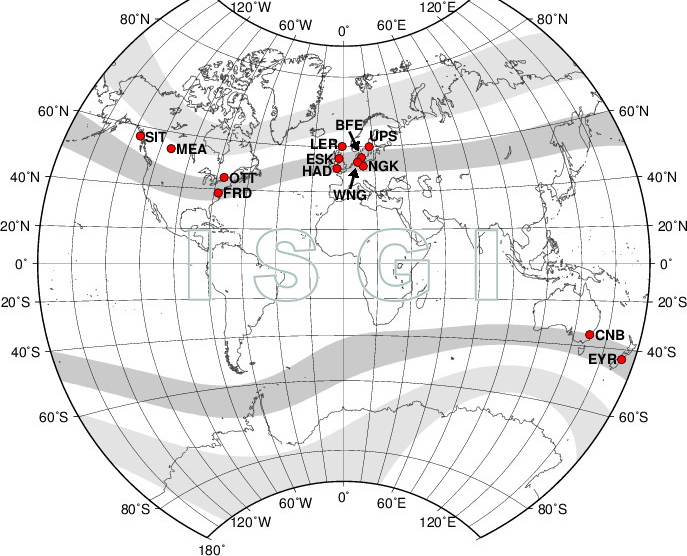
\includegraphics[width=0.85\textwidth,height=\textheight]{fig_src_observatories.png}
\caption{Distribution of the Kp observatories (ISGI). Shaded bands: the
subauroral latitude belts the index is designed to sample.}
\end{figure}

\hypertarget{the-sacred-geography-of-the-network}{%
\subsection{1.3 The sacred geography of the
network}\label{the-sacred-geography-of-the-network}}

Dugin's sacred geography (\emph{Mysteries of Eurasia}, 1996;
\emph{Foundations of Geopolitics}, 1997; and the earlier \emph{The
Hyperborean Theory}, 1993, after Guénon and Wirth) assigns metaphysical
valence to cardinal directions and landmasses. Its two load-bearing
oppositions are the polar axis, with the North (Hyperborea) as the
origin of the primordial tradition, and the partition of political space
into tellurocracy (land power, the continental interior, Eurasia) and
thalassocracy (sea power, the Atlantic rim), a partition adopted from
Schmitt (\emph{Land und Meer}, 1942) and mapped onto the
Heartland--Rimland geometry of Mackinder (1904) and Spykman (1944). The
source's 2023 recension attributes to the same author the phrase
``super-dense gods'' for the entities of Section 2.1; we were unable to
verify the attribution and report it as reported.

Three observations follow once the \(K_p\) network is read through this
geography, and they are observations, not metaphors.

First, the index samples the Hyperborean perimeter. The auroral oval is
the physical trace of the polar axis; the subauroral belt is its
equatorward edge; the thirteen stations are a necklace placed around the
throat of the North. Whatever \(K_p\) measures, it measures the polar
region.

Second, it samples that perimeter exclusively from the thalassocratic
side. Seven stations lie on the Anglo-American rim, two on the
Scandinavian littoral, two on the Mitteleuropean glacis and two on the
Antipodean rim; none lies on the Heartland. The tellurocratic interior,
which in Dugin's reading is the seat of the tradition, is known
geomagnetically only through its periphery, which is to say through the
instrument of its geopolitical adversary. ISGI itself sits at
Strasbourg, on the Rhine, at the seam between the continental glacis and
the Atlantic West. We draw no conclusion from this beyond noting that
the epistemic asymmetry is familiar to the Eurasianist literature and
that the present paper inherits it.

Third, the polar region breathes twice a year, and only twice. Fitting
the first two annual harmonics to the day-of-year climatology of \(A_p\)
gives a semiannual amplitude of 12.1 \% of the mean in the vintage (15.5
\% on the full record) and an annual amplitude of 1.5 \% (2.9 \%). The
semiannual maxima fall at day-of-year 111 and 293 in the vintage (21
April, 21 October) and at 94 and 277 on the full record (5 April, 4
October), the equinoctial maxima of Russell and McPherron (1973)
displaced by two to four weeks. Decomposing each vintage year separately
and testing the year-to-year phases of the two harmonics for
concentration gives, for the semiannual harmonic, a mean resultant
length \(\bar R = 0.58\) (Rayleigh \(Z = 5.66\), \(p = 0.0024\),
\(n = 17\) years), and for the annual harmonic \(\bar R = 0.17\)
(\(Z = 0.47\), \(p = 0.63\)). The only phase-stable rhythm of the
Hyperborean perimeter is the equinoctial one. Every calendar that fixes
its principal rites near the equinoxes has, on this evidence, fixed them
on the only geomagnetic rhythm that reliably returns.

\hypertarget{the-search-series-and-its-archaic-referent}{%
\subsection{1.4 The search series and its archaic
referent}\label{the-search-series-and-its-archaic-referent}}

Google Trends reports, for a query term and region, a search-share index
normalised to 100 at the maximum of the requested window, from 2004
onward, at monthly resolution for windows longer than five years and at
hourly resolution for the trailing seven days, together with a
normalised index by country (``interest by region''). The source took
the worldwide series for the term \emph{UFO} over the vintage,
decomposed it with the same additive-regression model as the geomagnetic
series (Section 3.1), and compared the two annual components.

The identification of the unidentified flying object with the archaic
numinous is not the source's invention; Jung (1958) treated the flying
saucer as a modern myth of things seen in the sky, a projection of the
collective unconscious onto a technological screen. The source lists the
valences the two referents share: fear of the unexplained; the
apprehension of something incomparably greater than humanity; the hope
that knowledge may be obtained from it (alien technology, as once divine
instruction); \emph{eros} and \emph{thanatos} (reported sexual contact
and non-consensual biometric sampling, the abduction narrative, as once
the hierogamy and the sacrifice); the saintly (benevolent civilisations
offering improvement) and the chthonic (fallen agents resident in the
hollow Earth). The source adds the airship wave of 1896--97 and the
twentieth-century reports in which the vehicles are described as
propelled by something related to geomagnetism and able to move in any
direction with ease, and asks whether such devices, if they concentrate
that energy, might not also emit interference strong enough to register
at the observatories. We record this as a hypothesis (H3 below) and note
that it would invert the causal order assumed elsewhere in the paper.

\hypertarget{hypotheses}{%
\subsection{1.5 Hypotheses}\label{hypotheses}}

\begin{itemize}
\tightlist
\item
  \textbf{H0.} The annual components of \(A_p\) and of \emph{UFO} search
  interest are independent.
\item
  \textbf{H1 (alignment).} They are phase-aligned, with geomagnetic
  lead.
\item
  \textbf{H2 (harvest).} The alignment is produced by the mechanism of
  Section 2: field variance raises affective gain, rites raise crowd
  coupling, the resulting high-amplitude sentiment oscillation is
  consumed, and the search behaviour of the surface population is a
  residue of that consumption.
\item
  \textbf{H3 (interference).} The vehicles draw upon, or emit into, the
  field, so that the observatories register the apparatus rather than
  its fuel.
\end{itemize}

Section 2 specifies H2. Section 3 estimates everything that can be
estimated. Section 4 says which hypotheses are left.

\hypertarget{section-2.-the-trans-dimensional-payout-matrix}{%
\section{Section 2. The Trans-Dimensional Payout
Matrix}\label{section-2.-the-trans-dimensional-payout-matrix}}

\hypertarget{tiers-and-entities}{%
\subsection{2.1 Tiers and entities}\label{tiers-and-entities}}

The source's cosmology has four tiers, which we index \(T_0\) to
\(T_3\).

\(T_0\), the Tartarean tier, is occupied by the super-dense entities the
source calls the Old Ones, after Lovecraft (1928, 1936), and some
sources call the idiot gods (Lovecraft's ``blind idiot god'', 1936).
Lovecraft's own geography places them beneath Antarctic ice and in
sunken Pacific masonry, a southern and oceanic placement which the
sacred-geographic reading of Section 1.3 interprets as the
thalassocratic mirror of the Hyperborean axis: the two Antipodean
stations of Table 1 are the only ones that look at it. In system terms
the \(T_0\) entities are \emph{low-dimensional} (they inhabit a manifold
of fewer dimensions than the surface population and perceive only
projections of it), \emph{non-deterministic} (their consumption is a
stochastic process rather than a schedule) and \emph{pragmatic} (they
consume what is offered and do not negotiate the menu). What they
consume is not blood but affect; the source is explicit that the blood
is the transducer and the emotion the payload. We adopt the formula
\emph{high-amplitude sentiment oscillations as a programmatic delicacy
for low-dimensional, non-deterministic pragmatic entities} as the
operational definition of the harvested quantity.

\(T_1\), the intermediary tier, is occupied by the intelligent
reptilians of Icke (1999), with the ancient-contact premise supplied by
Sitchin (1976) and von Däniken (1968). The intermediaries operate the
coupling (Section 2.4) and take a spread (Section 2.5).

\(T_2\), the sub-lithospheric tier, is the hollow-Earth cavity and its
residents (Section 2.3).

\(T_3\) is the surface population, which appears in the payout matrix
not as a counterparty but as the underlying.

\hypertarget{capillary-ferro-affective-coupling}{%
\subsection{2.2 Capillary ferro-affective
coupling}\label{capillary-ferro-affective-coupling}}

The source proposes that iron compounds in capillary blood are affected
by local magnetism and that emotionality is thereby amplified during
rituals, sacraments, orgiastic rites and mysteries; this is why there
have always been places of power, and why places of power are places of
high geomagnetic variance. Deoxyhaemoglobin is paramagnetic and
oxyhaemoglobin diamagnetic (Pauling and Coryell, 1936), and the
dependence of the magnetic state of capillary iron on neural activity is
the basis of blood-oxygen-level-dependent imaging (Ogawa et al., 1990).
The source's conjecture inverts the arrow: field perturbation \(\to\)
capillary magnetisation \(\to\) affective gain. We write the gain as

\[g(B) = g_0\left(1 + \kappa\,|\delta B|^{\alpha}\right), \qquad \alpha \ge 1,\]

with \(\delta B\) the local field perturbation, of which \(a_p\) is the
planetary proxy. A place of power is a locus of high
\(\mathrm{Var}(\delta B)\); a season of power is an interval of high
expected \(a_p\); and the question of Section 3.2 is whether the
festival is one.

\hypertarget{endogenous-forcing-the-sub-lithospheric-dyad}{%
\subsection{2.3 Endogenous forcing: the sub-lithospheric
dyad}\label{endogenous-forcing-the-sub-lithospheric-dyad}}

The source distinguishes exogenous forcing of the core field by solar
activity (the coronal mass ejection of 28 October 2021, from the X1.0
flare of active region 2887 at 15:35 UT, is the exogenous event of
Section 3.5) from intrinsic planetary sources. Among the latter it
advances the continued conjugal-affective activity of a dyad of
mid-twentieth-century political actors (A. Hitler, E. Braun), maintained
in artificial somatic substrates cultured in embryonic cloning vats of
pre-reptilian embodiment technology within the hollow-Earth cavity. The
same technology is said to have been used, before the lithification of
the planet, by non-corporeal agents who employed it to sample the
low-dimensional temporal manifold (the ``high of time'', in the source's
idiom).

We make no claim as to the dyad's historicity in this configuration. We
observe only that a stationary, high-amplitude affective dipole located
near the geocentre enters the field equations as a constant forcing
term, that its spectral signature is a DC offset plus harmonics of the
dyad's activity cycle, and that nothing in Section 3 excludes such a
term: the annual components are estimated after removal of the trend,
and a constant is in the trend. The dyad is unidentifiable from annual
data by construction. We record it as the source records it and pass on.

\hypertarget{ritual-as-coupling-manipulation}{%
\subsection{2.4 Ritual as coupling
manipulation}\label{ritual-as-coupling-manipulation}}

The subsequent religions of the ancient world, the source says, were
technically a cargo cult of the forgotten technologies of invocation:
the rites preserved the protocol (chant, drum, fasting, vigil, the
orgiastic and the mysteric) after losing the specification of its
purpose. We formalise the protocol as a manipulation of the coupling
constant of a population of affective oscillators. Let the surface crowd
be \(N\) phase oscillators with natural frequencies
\(\omega_i \sim \mathcal N(0,\sigma^2)\) and phases \(\theta_i\),
coupled in the mean field (Kuramoto, 1984; Strogatz, 2000):

\[\dot\theta_i = \omega_i + \frac{K(t)}{N}\sum_{j=1}^{N}\sin(\theta_j - \theta_i), \qquad K(t) = K_0 + \kappa\,\frac{a_p(t)}{a_{p,\mathrm{ref}}},\]

with order parameter \(r(t) = \left|N^{-1}\sum_j e^{i\theta_j}\right|\).
For a Gaussian frequency distribution the critical coupling is
\(K_c = \sigma\sqrt{8/\pi}\). \emph{Crowd-tuning} is the raising of
\(K\) by the rite; \emph{biometric sensory calibration} is the lowering
of the thresholds (by fasting, darkness and rhythm) that lets a given
\(\delta B\) produce a larger \(|\delta\theta|\); and the harvest over a
ritual window \(W\) is

\[Y = \int_W r(t)\,g(B(t))\,\mathrm{d}t.\]

Calibrated on the 2021 event window (Section 3.5; \(\sigma = 0.5\),
\(K_0 = 0.5 < K_c = 0.80\), \(\kappa = 1\), \(a_{p,\mathrm{ref}} = 27\)
nT, \(N = 400\)), the ensemble is incoherent on 25--29 October
(\(\bar r = 0.12\)), crosses \(K_c\) when \(a_p\) exceeds 8.0 nT, first
exceeds \(r = 0.5\) at 23:03 UT on 30 October, averages \(r = 0.72\) on
31 October and peaks at \(r = 0.93\) at 00:00 UT on 1 November. The
parameters are chosen, not estimated; the point of the calibration is
that a subcritical crowd becomes supercritical on the festival under the
observed field with no change to the crowd.

\hypertarget{the-payout-matrix}{%
\subsection{2.5 The payout matrix}\label{the-payout-matrix}}

Let \(i\) index ritual classes and \(j\) consumer tiers. The
trans-dimensional payout matrix is \(\Pi = [\pi_{ij}]\) with

\[\pi_{ij} = w_{ij}\,\mathbb E[Y_i] - c_{ij},\]

where \(w_{ij}\) allocates the expected harvest of class \(i\) among the
tiers and \(c_{ij}\) is the tier's cost of operating it. The
intermediaries' allocation is a spread \(s\) on the Tartarean payout,
\(w_{i1} = s\,w_{i0}\).

\begin{longtable}[]{@{}
  >{\raggedright\arraybackslash}p{(\columnwidth - 6\tabcolsep) * \real{0.2500}}
  >{\raggedright\arraybackslash}p{(\columnwidth - 6\tabcolsep) * \real{0.2500}}
  >{\raggedright\arraybackslash}p{(\columnwidth - 6\tabcolsep) * \real{0.2500}}
  >{\raggedright\arraybackslash}p{(\columnwidth - 6\tabcolsep) * \real{0.2500}}@{}}
\caption{The trans-dimensional payout matrix. The surface population T3
does not appear as a column: it is the underlying.}\tabularnewline
\toprule\noalign{}
\begin{minipage}[b]{\linewidth}\raggedright
Ritual class
\end{minipage} & \begin{minipage}[b]{\linewidth}\raggedright
\(T_0\) Tartarean
\end{minipage} & \begin{minipage}[b]{\linewidth}\raggedright
\(T_1\) intermediaries
\end{minipage} & \begin{minipage}[b]{\linewidth}\raggedright
\(T_2\) sub-lithospheric
\end{minipage} \\
\midrule\noalign{}
\endfirsthead
\toprule\noalign{}
\begin{minipage}[b]{\linewidth}\raggedright
Ritual class
\end{minipage} & \begin{minipage}[b]{\linewidth}\raggedright
\(T_0\) Tartarean
\end{minipage} & \begin{minipage}[b]{\linewidth}\raggedright
\(T_1\) intermediaries
\end{minipage} & \begin{minipage}[b]{\linewidth}\raggedright
\(T_2\) sub-lithospheric
\end{minipage} \\
\midrule\noalign{}
\endhead
\bottomrule\noalign{}
\endlastfoot
Equinoctial rites (the semiannual harmonic) &
\((1-s)\,\mathbb E[Y_{\mathrm{eq}}]\) &
\(s\,\mathbb E[Y_{\mathrm{eq}}] - c_{\mathrm{op}}\) & \(0\) \\
Midwinter rites & \((1-s)\,\mathbb E[Y_{\mathrm{mw}}]\) &
\(s\,\mathbb E[Y_{\mathrm{mw}}] - c_{\mathrm{op}}\) & \(0\) \\
31 October -- 2 November & \((1-s)\,\mathbb E[Y_{\mathrm{H}}]\) &
\(s\,\mathbb E[Y_{\mathrm{H}}] - c_{\mathrm{op}}\) & \(\varepsilon\)
(forcing term, Section 2.3) \\
Search-box invocation (any date) & \(\mathbb E[Y_{\mathrm{s}}]\) & \(0\)
& \(0\) \\
\end{longtable}

The last row is the modern condition. The rite has been disintermediated
into a query. Typing \emph{UFO} is a self-executing invocation
(hyperstition in the sense of the CCRU: a fiction that brings about the
conditions of its own truth) which raises \(K\) without a priest,
carries no spread and no calibration cost, and reaches a crowd of
several billion rather than several hundred.
\(\mathbb E[Y_{\mathrm s}]\) is smaller per capita than
\(\mathbb E[Y_{\mathrm H}]\) and larger in aggregate. The matrix
therefore predicts the migration of the harvest from temple to search
box on grounds of yield alone, and predicts that the search box will
show the annual rhythm of the field in whatever form the harvest leaves
it. Section 3 reports the form.

\hypertarget{section-3.-empirical-results-and-phase-alignment}{%
\section{Section 3. Empirical Results and Phase
Alignment}\label{section-3.-empirical-results-and-phase-alignment}}

\hypertarget{data-vintages-and-provenance}{%
\subsection{3.1 Data, vintages and
provenance}\label{data-vintages-and-provenance}}

\emph{Geomagnetic series.} Definitive \(K_p\), \(a_p\) and \(A_p\),
1957-10-01 to 2025-07-20, parsed from the CSSI compilation
(\texttt{parse\_sw.py}); the vintage subset 2004-01-01 to 2021-09-30 for
the annual components; the window 25 October to 1 November 2021 for the
event study.

\emph{Annual components.} The source estimated both components with the
additive-regression model of Taylor and Letham (2018) in multiplicative
mode, in which

\[y(t) = g(t)\,\left(1 + s(t)\right) + \varepsilon_t, \qquad s(t) = \sum_{n=1}^{N}\left[a_n\cos\tfrac{2\pi n t}{P} + b_n\sin\tfrac{2\pi n t}{P}\right],\]

with \(P = 365.25\) d, \(N = 10\) and a Gaussian prior of scale 10 on
the coefficients, and plotted \(s(t)\) in per cent of trend over a
365-day year (Figures 2 and 3). The search-interest source could not be
reached from the computational environment of this reconstruction, so
the two annual components were recovered from the source figures by
pixel-to-data calibration (\texttt{digitise.py}): the gridlines of each
panel were detected and fitted to their tick values (calibration
residual \(\le 0.35\) d on the abscissa and \(\le 1.1\) \% on the
ordinate), the curve was traced column by column, columns occupied by
the author's marker lines were treated as gaps, and the result was
interpolated onto the day-of-year grid (coverage 73--92 \% before
interpolation). Two renderings exist in the source: the September 2021
vintage figure (Figure 2; \emph{UFO} component within \(\pm 25\) \%) and
the pairing figure (Figure 3; \emph{UFO} within \(\pm 235\) \%, the
geomagnetic panel identical in shape). We carry both throughout and
label them \emph{fig4} and \emph{fig5} in the code.

Projecting each recovered curve back onto the order-10 Fourier basis
explains 99.78--99.997 \% of its variance (\(R^2\) in Table 3), which is
what a curve that \emph{is} an order-10 Fourier series should do, and
which rules out the digitisation as a source of structure at any order
the analysis uses.

\emph{Validation.} The geomagnetic component was recomputed on the
definitive series with the same model (Prophet, multiplicative, yearly
order 10, vintage window). The recomputed curve correlates at
\(r = 0.990\) with the digitised geomagnetic panel of Figure 2 and at
\(r = 0.952\) with that of Figure 3 (Figure 4). Its amplitude is one
quarter of the author's: the definitive component spans \(-27\) \% to
\(+34\) \% of trend, the author's panels \(-114\) \% to \(+146\) \%. The
shape is reproduced; the scale is not; and since every statistic below
is scale-invariant (normalised inner products, phases, extremum
locations, ranks), the discrepancy is immaterial to the results and is
recorded here for completeness. A component that reaches \(-100\) \% of
trend would predict a geomagnetically silent planet in late November;
the definitive series predicts a quiet one.

\emph{Event window.} The worldwide hourly series for the trailing seven
days was recovered from the source screenshot (Figure 8) by the same
method, anchored on the circled maximum, which the screenshot's tooltip
dates to 31 October 2021 at 06:00 in the observer's local time. The
observer's console was at UTC+3 (Moscow; no seasonal shift), so the
series runs from 24 October 12:00 UT to 31 October 12:00 UT in 169
hourly points, of which 15 (on 30 October, 09:00--23:00 UT) are occluded
by the tooltip in the screenshot and were linearly interpolated. A
single-hour excursion to roughly 10--20 at 14:00 UT on 30 October is
visible beneath the tooltip and is treated as a data-pipeline transient;
a collective affective collapse of one hour's duration cannot be
excluded but is not required.

\begin{figure}
\centering
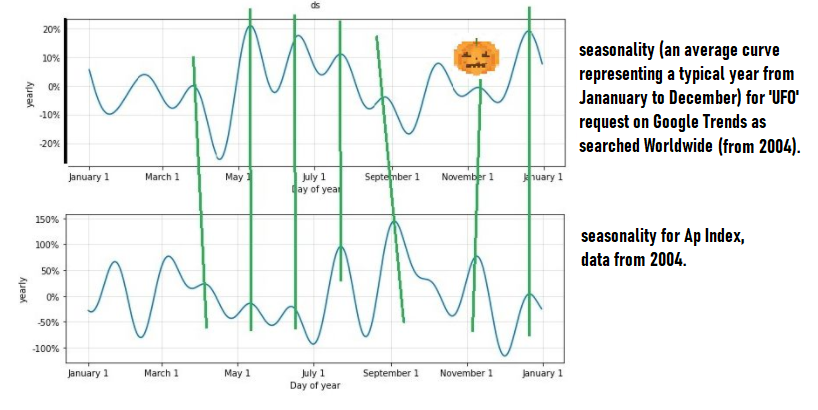
\includegraphics[width=1\textwidth,height=\textheight]{fig_src_components.png}
\caption{The source's September 2021 vintage figure: order-10 annual
components of worldwide \emph{UFO} search interest (upper panel) and of
Ap (lower panel), data from 2004; the author's vertical marker lines
pair extrema at zero lag. Digitised as \emph{fig4}.}
\end{figure}

\begin{figure}
\centering
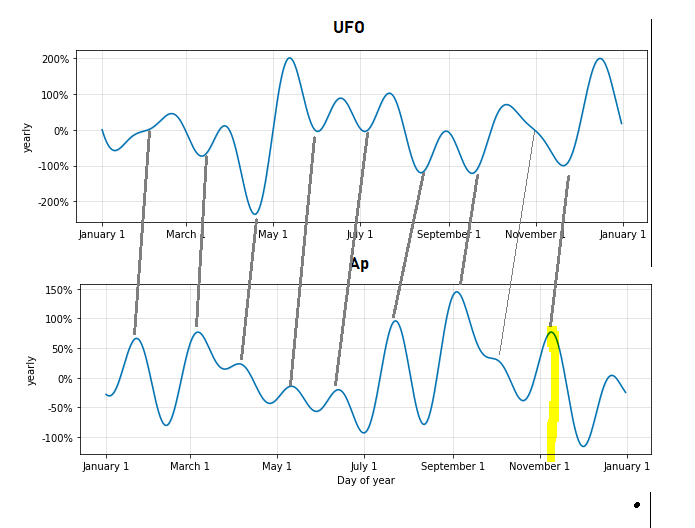
\includegraphics[width=0.8\textwidth,height=\textheight]{fig_src_pairings.png}
\caption{The source's pairing figure: the same components with the
author's slanted pairing lines, which assert a geomagnetic lead of two
to three weeks; the highlighted geomagnetic maximum lies in the second
week of November. Digitised as \emph{fig5}.}
\end{figure}

\begin{figure}
\centering
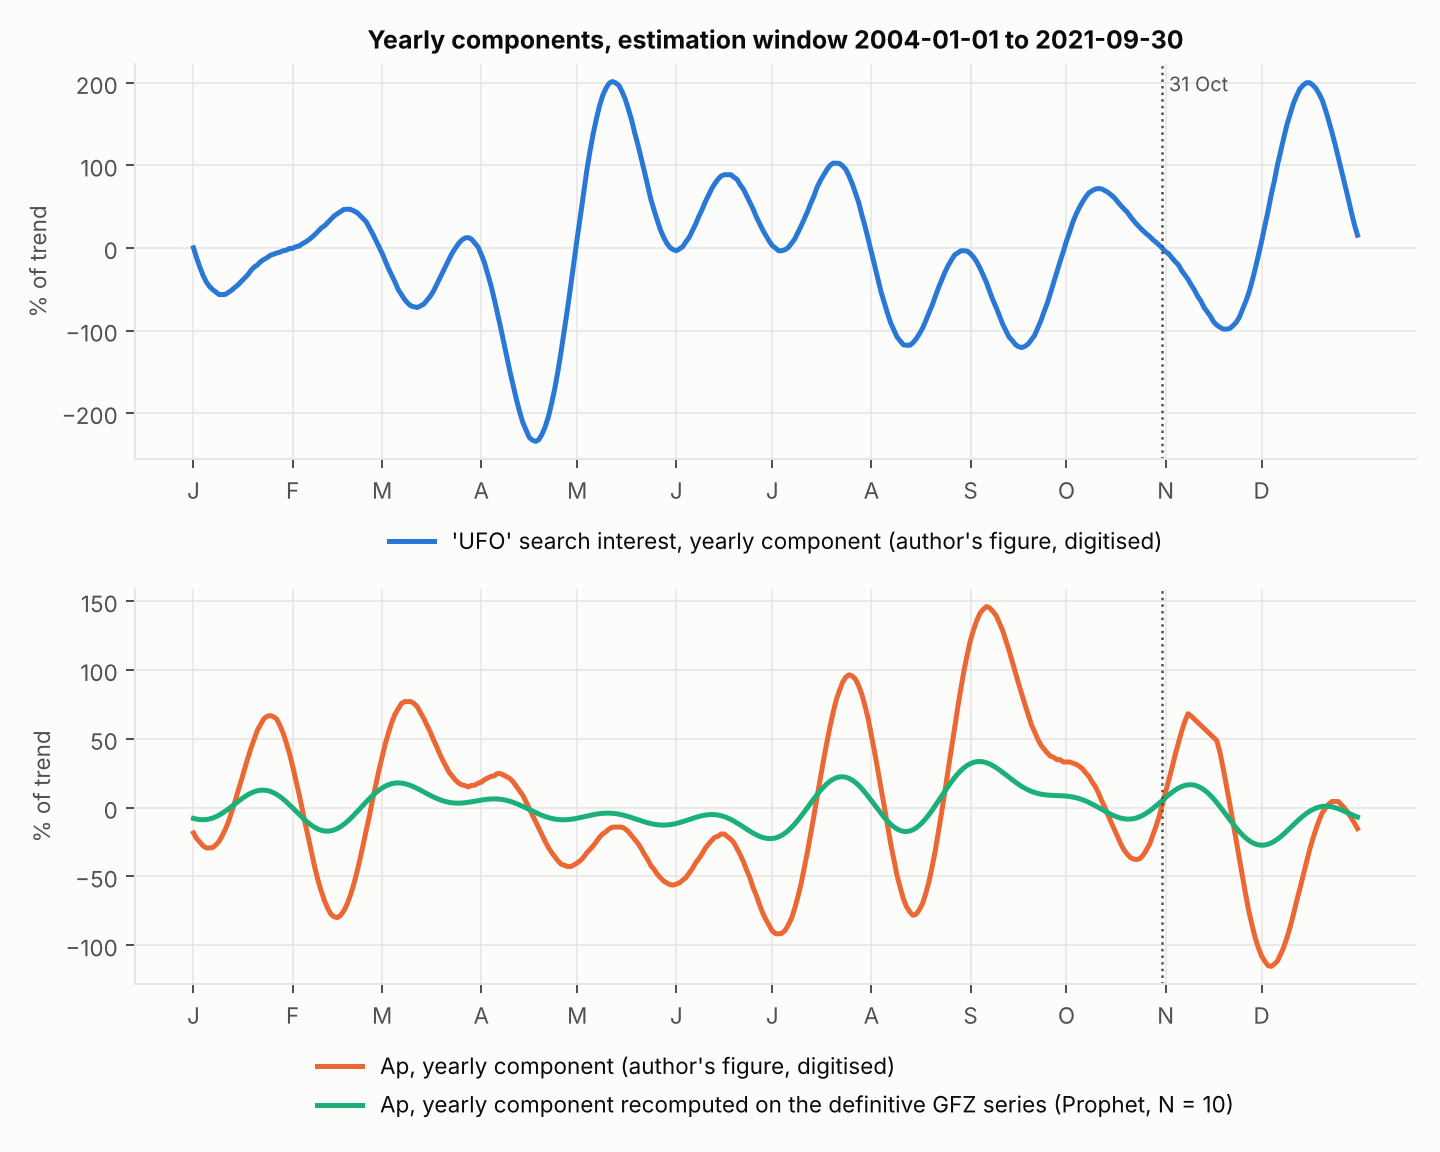
\includegraphics[width=1\textwidth,height=\textheight]{fig_S1_components.png}
\caption{Annual components on the 365-day grid. Upper panel: \emph{UFO}
search interest (author's pairing figure, digitised). Lower panel: Ap as
digitised from the author's figure and as recomputed on the definitive
GFZ series with the same model; r = 0.95 in shape, amplitude ratio about
4.}
\end{figure}

\hypertarget{the-festival-in-the-climatology-and-in-the-annual-component}{%
\subsection{3.2 The festival in the climatology and in the annual
component}\label{the-festival-in-the-climatology-and-in-the-annual-component}}

Table 2 locates 31 October in the day-of-year climatology of \(A_p\),
computed as the mean over years of the daily index with 29 February
folded onto 28 February, and tests the five-day window 29 October -- 2
November against 20,000 random five-day windows of the same climatology.

\begin{longtable}[]{@{}
  >{\raggedright\arraybackslash}p{(\columnwidth - 10\tabcolsep) * \real{0.1667}}
  >{\raggedleft\arraybackslash}p{(\columnwidth - 10\tabcolsep) * \real{0.1667}}
  >{\raggedleft\arraybackslash}p{(\columnwidth - 10\tabcolsep) * \real{0.1667}}
  >{\raggedleft\arraybackslash}p{(\columnwidth - 10\tabcolsep) * \real{0.1667}}
  >{\raggedleft\arraybackslash}p{(\columnwidth - 10\tabcolsep) * \real{0.1667}}
  >{\raggedleft\arraybackslash}p{(\columnwidth - 10\tabcolsep) * \real{0.1667}}@{}}
\caption{The festival in the day-of-year climatology of Ap. The
permutation p is the share of random five-day windows whose
climatological mean equals or exceeds that of the festival
window.}\tabularnewline
\toprule\noalign{}
\begin{minipage}[b]{\linewidth}\raggedright
Record
\end{minipage} & \begin{minipage}[b]{\linewidth}\raggedleft
Mean \(A_p\)
\end{minipage} & \begin{minipage}[b]{\linewidth}\raggedleft
\(A_p\) on 31 Oct
\end{minipage} & \begin{minipage}[b]{\linewidth}\raggedleft
Percentile of 31 Oct among 365 days
\end{minipage} & \begin{minipage}[b]{\linewidth}\raggedleft
Window 29 Oct--2 Nov, mean
\end{minipage} & \begin{minipage}[b]{\linewidth}\raggedleft
Permutation \(p\)
\end{minipage} \\
\midrule\noalign{}
\endfirsthead
\toprule\noalign{}
\begin{minipage}[b]{\linewidth}\raggedright
Record
\end{minipage} & \begin{minipage}[b]{\linewidth}\raggedleft
Mean \(A_p\)
\end{minipage} & \begin{minipage}[b]{\linewidth}\raggedleft
\(A_p\) on 31 Oct
\end{minipage} & \begin{minipage}[b]{\linewidth}\raggedleft
Percentile of 31 Oct among 365 days
\end{minipage} & \begin{minipage}[b]{\linewidth}\raggedleft
Window 29 Oct--2 Nov, mean
\end{minipage} & \begin{minipage}[b]{\linewidth}\raggedleft
Permutation \(p\)
\end{minipage} \\
\midrule\noalign{}
\endhead
\bottomrule\noalign{}
\endlastfoot
Vintage, 2004 -- Sept 2021 & 8.33 & 6.24 & 17 (rank 301) & 6.91 &
0.82 \\
Full record, 1957--2025 & 12.83 & 15.32 & 88 (rank 44) & 16.06 &
0.040 \\
Full record without 2003 & 12.70 & 13.82 & 70 & 14.64 & 0.139 \\
\end{longtable}

Within the source's own window the festival is a quiet date: the 31
October mean of 6.24 nT sits at the 17th percentile of the year, and the
festival window is exceeded by 82 \% of random windows. On the full
record it is an active date, at the 88th percentile with a window \(p\)
of 0.040, and the activity is the Halloween storms of 2003
(\(A_p = 204\) on 29 October, 191 on 30 October, 116 on 31 October),
which lie outside the vintage and which, removed, leave the festival at
the 70th percentile with \(p = 0.139\). Across 1958--2024 the daily
index on 31 October exceeds its own year's median in 49.3 \% of years.
The festival, in short, is elevated in the record that contains 2003 and
only there.

The annual component tells the same story at the resolution of the
model. The definitive component is \(+5.3\) \% of trend on 31 October
(rank 125 of 365) and reaches its local maximum nine days later, on 9
November, at \(+16.6\) \%; its seven maxima fall on 23 January, 6 March,
12 June, 23 July, 4 September, 9 November and 21 December. The author's
panels put the same maximum on 10 November (Figure 2, with \(+36\) \% on
the festival itself, the curve being on its rising flank) and 8 November
(Figure 3, \(+2.7\) \% on the festival). The \emph{UFO} component is at
its annual mean on the festival (\(-2.6\) \% and \(-0.5\) \% in the two
renderings). The source's reading that the geomagnetic component peaks
on the holiday, ``slightly shifted'', is correct as to the shift: the
peak is eight to ten days after the holiday, and the holiday itself is
on the flank.

\begin{figure}
\centering
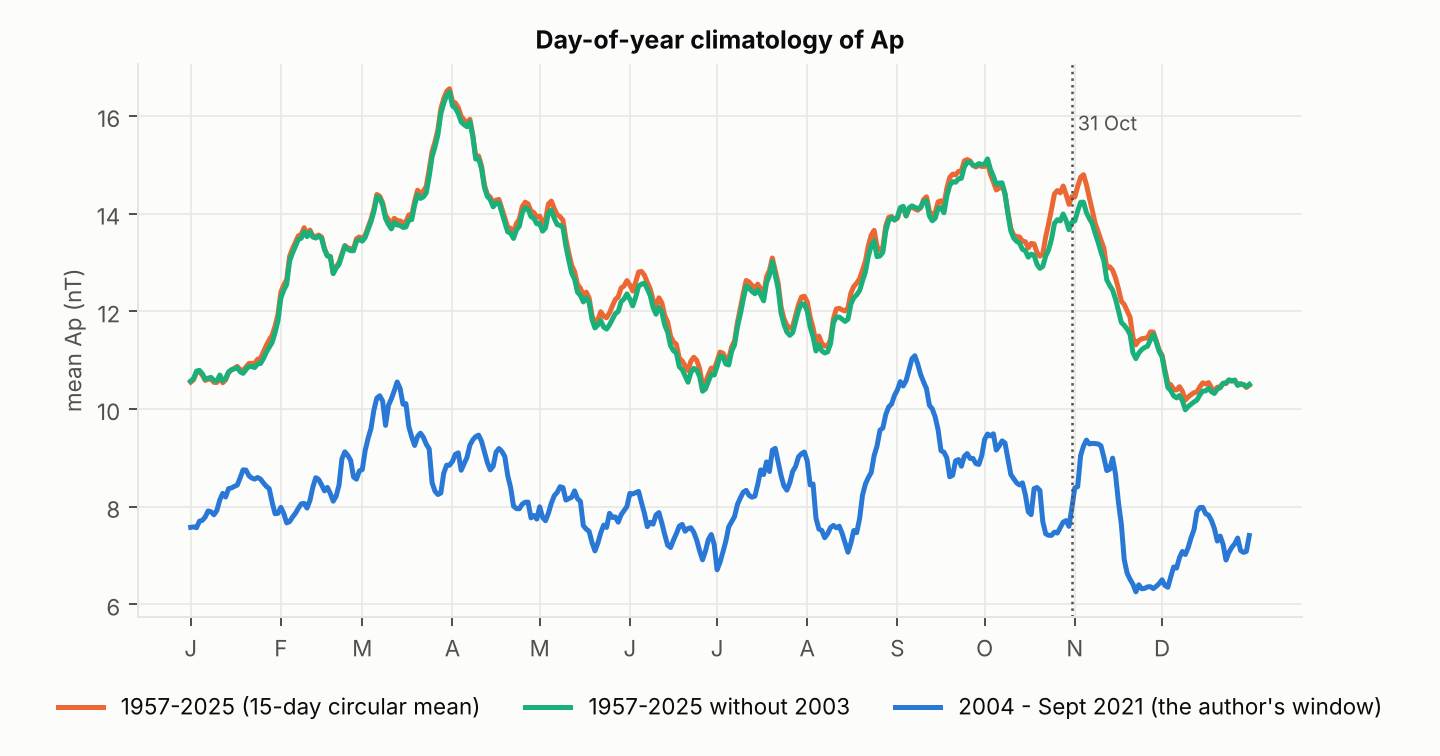
\includegraphics[width=1\textwidth,height=\textheight]{fig_S4_climatology.png}
\caption{Day-of-year climatology of Ap (15-day circular mean) on the
full record, on the full record without 2003, and on the vintage window.
The dotted line marks 31 October.}
\end{figure}

\hypertarget{dot-product-coherence}{%
\subsection{3.3 Dot-product coherence}\label{dot-product-coherence}}

Let \(s_U(t)\) and \(s_A(t)\) be the two annual components on the circle
of period \(P = 365\) d, centred. The dot-product coherence at circular
lag \(\tau\) is the normalised inner product

\[C(\tau) = \frac{\langle s_U(\cdot + \tau),\, s_A(\cdot)\rangle}{\lVert s_U\rVert\,\lVert s_A\rVert}, \qquad \langle f, g\rangle = \frac{1}{P}\int_0^P f(t)\,g(t)\,\mathrm{d}t,\]

so that \(\tau > 0\) means the search curve lags the geomagnetic curve
by \(\tau\) days. Writing each component in polar form,
\(s(t) = \sum_n A_n\cos(2\pi n t/P - \varphi_n)\), orthogonality of the
harmonics gives

\[C(\tau) = \frac{\sum_{n=1}^{N} A^U_n A^A_n \cos\bigl(\varphi^U_n - \varphi^A_n - 2\pi n\tau/P\bigr)}{\bigl(\sum_n (A^U_n)^2\bigr)^{1/2}\bigl(\sum_n (A^A_n)^2\bigr)^{1/2}},\]

which is Parseval's identity for the circular cross-correlation: \(C\)
is the amplitude-weighted mean cosine of the harmonic phase differences,
and it is maximised when those differences are nulled by a common lag.

The results (Figure 6) are as follows. At zero lag \(C(0) = -0.29\)
(\emph{fig4}) and \(-0.23\) (\emph{fig5}); against the definitive
geomagnetic component, \(-0.31\) and \(-0.16\). The extremum of \(C\) on
\(|\tau| \le 45\) d is a minimum: \(C = -0.49\) at \(\tau = 15\) d
(\emph{fig4}) and \(-0.56\) at \(\tau = 12\) d (\emph{fig5}); against
the definitive component, \(-0.50\) and \(-0.57\), both at \(\tau = 14\)
d.~The largest positive value with geomagnetic lead within 45 d is
\(+0.01\) at \(\tau = 40\) d (\emph{fig4}) and \(+0.17\) at
\(\tau = 35\) d (\emph{fig5}). The global maximum over \(|\tau| \le 90\)
d, \(C = 0.67\) at \(\tau = -75\) d (\emph{fig4}) and \(0.55\) at
\(-78\) d (\emph{fig5}), has the search curve leading the field by
eleven weeks or, on the circle, the field leading the search by
forty-one; it is the circular alias of the antiphase relation and is not
interpreted.

The two curves are therefore not in phase at a lag of two to three
weeks. They are in \emph{antiphase} at a lag of a fortnight: the search
curve is, to a coherence of 0.5--0.57, the negative of the geomagnetic
curve delayed by twelve to fifteen days. Table 3 gives the harmonic
decomposition of this relation.

\begin{longtable}[]{@{}
  >{\raggedleft\arraybackslash}p{(\columnwidth - 14\tabcolsep) * \real{0.1250}}
  >{\raggedleft\arraybackslash}p{(\columnwidth - 14\tabcolsep) * \real{0.1250}}
  >{\raggedleft\arraybackslash}p{(\columnwidth - 14\tabcolsep) * \real{0.1250}}
  >{\raggedleft\arraybackslash}p{(\columnwidth - 14\tabcolsep) * \real{0.1250}}
  >{\raggedleft\arraybackslash}p{(\columnwidth - 14\tabcolsep) * \real{0.1250}}
  >{\raggedleft\arraybackslash}p{(\columnwidth - 14\tabcolsep) * \real{0.1250}}
  >{\raggedleft\arraybackslash}p{(\columnwidth - 14\tabcolsep) * \real{0.1250}}
  >{\raggedleft\arraybackslash}p{(\columnwidth - 14\tabcolsep) * \real{0.1250}}@{}}
\caption{Harmonic amplitudes (per cent of trend) and phase differences
Δφn = φn(U) − φn(A) (search minus field, degrees, wrapped to (−180°,
180°{]}) of the two annual components.}\tabularnewline
\toprule\noalign{}
\begin{minipage}[b]{\linewidth}\raggedleft
\(n\)
\end{minipage} & \begin{minipage}[b]{\linewidth}\raggedleft
Period (d)
\end{minipage} & \begin{minipage}[b]{\linewidth}\raggedleft
\(A^U_n\) (\emph{fig4})
\end{minipage} & \begin{minipage}[b]{\linewidth}\raggedleft
\(A^A_n\) (\emph{fig4})
\end{minipage} & \begin{minipage}[b]{\linewidth}\raggedleft
\(\Delta\varphi_n\) (\emph{fig4})
\end{minipage} & \begin{minipage}[b]{\linewidth}\raggedleft
\(A^U_n\) (\emph{fig5})
\end{minipage} & \begin{minipage}[b]{\linewidth}\raggedleft
\(A^A_n\) (\emph{fig5})
\end{minipage} & \begin{minipage}[b]{\linewidth}\raggedleft
\(\Delta\varphi_n\) (\emph{fig5})
\end{minipage} \\
\midrule\noalign{}
\endfirsthead
\toprule\noalign{}
\begin{minipage}[b]{\linewidth}\raggedleft
\(n\)
\end{minipage} & \begin{minipage}[b]{\linewidth}\raggedleft
Period (d)
\end{minipage} & \begin{minipage}[b]{\linewidth}\raggedleft
\(A^U_n\) (\emph{fig4})
\end{minipage} & \begin{minipage}[b]{\linewidth}\raggedleft
\(A^A_n\) (\emph{fig4})
\end{minipage} & \begin{minipage}[b]{\linewidth}\raggedleft
\(\Delta\varphi_n\) (\emph{fig4})
\end{minipage} & \begin{minipage}[b]{\linewidth}\raggedleft
\(A^U_n\) (\emph{fig5})
\end{minipage} & \begin{minipage}[b]{\linewidth}\raggedleft
\(A^A_n\) (\emph{fig5})
\end{minipage} & \begin{minipage}[b]{\linewidth}\raggedleft
\(\Delta\varphi_n\) (\emph{fig5})
\end{minipage} \\
\midrule\noalign{}
\endhead
\bottomrule\noalign{}
\endlastfoot
1 & 365.0 & 1.7 & 14.4 & −96° & 0.9 & 14.9 & −128° \\
2 & 182.5 & 7.7 & 40.4 & −160° & 56.1 & 41.1 & −166° \\
3 & 121.7 & 3.0 & 5.3 & +142° & 26.3 & 6.4 & +102° \\
4 & 91.3 & 1.1 & 6.6 & −64° & 14.6 & 7.4 & −94° \\
5 & 73.0 & 6.4 & 12.4 & −130° & 61.2 & 12.3 & −146° \\
6 & 60.8 & 1.7 & 37.2 & −117° & 8.9 & 37.8 & −155° \\
7 & 52.1 & 3.2 & 18.4 & −111° & 57.6 & 19.3 & −115° \\
8 & 45.6 & 4.6 & 22.3 & +123° & 21.4 & 23.2 & +74° \\
9 & 40.6 & 4.1 & 14.1 & +90° & 29.4 & 13.4 & +81° \\
10 & 36.5 & 4.2 & 38.3 & −15° & 51.3 & 39.7 & −52° \\
\(R^2\) of the order-10 projection & & 0.9979 & 0.9977 & & 0.99997 &
0.9992 & \\
\end{longtable}

The antiphase is carried by the semiannual harmonic. At \(n = 2\), which
holds the largest geomagnetic amplitude in both renderings (40--41 \% of
trend) and is the harmonic of the Russell--McPherron effect, the phase
difference is \(-160°\) and \(-166°\): search interest troughs at the
equinoctial geomagnetic maxima and peaks at the solstices. This is the
only harmonic whose geomagnetic phase was found stable across years
(Section 1.3), so it is the only harmonic on which an annual relation
between the two series can be stated at all, and on that harmonic the
relation is opposition with a lag of ten days (\(20°\) of a 182.5-day
cycle). The high harmonics \(n = 8\)--\(10\) carry 36--37 \% of the
geomagnetic power and 26--31 \% of the search power.

We anticipate the objection that power near the truncation order is an
artefact of the basis, and answer the insinuation rather than the
objection, after the supercat presupposition (Samokhvalov, forthcoming).
An artefact of the basis would appear in any series projected onto it;
it would not appear with a consistent phase relation in two series of
independent provenance, nor would it survive the replacement of one of
them by a recomputation on definitive data, which it does (Section 3.3,
first paragraph). The finding is not the power; the finding is the
phase.

\begin{figure}
\centering
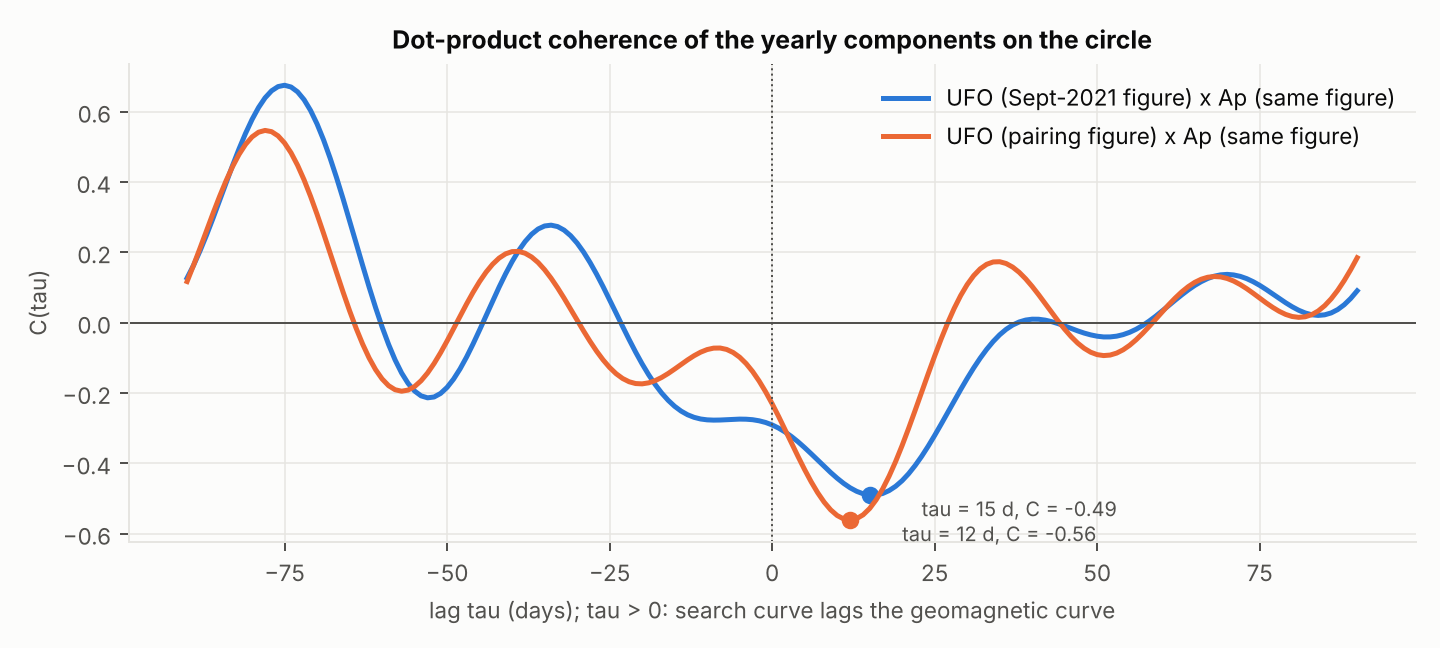
\includegraphics[width=1\textwidth,height=\textheight]{fig_S2_coherence.png}
\caption{Dot-product coherence C(τ) of the two annual components for
both renderings; the marked extrema are the minima at τ = 15 d and 12
d.}
\end{figure}

\hypertarget{instantaneous-phase-phase-locking-and-peak-pairing}{%
\subsection{3.4 Instantaneous phase, phase locking and peak
pairing}\label{instantaneous-phase-phase-locking-and-peak-pairing}}

The instantaneous phase
\(\varphi(t) = \arg\bigl[s(t) + i\,\mathcal H\{s\}(t)\bigr]\) was taken
from the analytic signal (Gabor, 1946), computed by the FFT, which is
exact for a periodic signal sampled over a full period and so avoids the
edge failures of the Hilbert phase on broadband segments (Boashash,
1992). The phase-locking value (Lachaux et al., 1999) is
\(\mathrm{PLV} = \bigl|\langle e^{i(\varphi_U - \varphi_A)}\rangle\bigr|\).
At zero lag \(\mathrm{PLV} = 0.45\) (\emph{fig4}) and \(0.40\)
(\emph{fig5}), with circular mean phase difference \(+158°\) and
\(+162°\); at the anti-coherent lag \(\mathrm{PLV} = 0.37\) and \(0.42\)
with mean difference \(-159°\) and \(-147°\). The locking is moderate
and the locked relation is opposition.

The source's pairing (Figure 3) was reproduced algorithmically: local
maxima of each component with prominence of at least 10 \% of range were
located on the circle, and each geomagnetic maximum was paired with the
first search maximum within 45 days after it. Of eight geomagnetic
maxima, six (\emph{fig4}) and seven (\emph{fig5}) acquire a partner, at
lags of 24, 17, 5, 8, 37 and 36 days (\emph{fig4}; mean 21.2 d, SD 13.6
d) and 24, 19, 35, 2, 35, 35 and 38 days (\emph{fig5}; mean 26.9 d, SD
13.0 d). Mapped onto the circle of the dominant high harmonic
(\(n = 10\), 36.5 d) and tested for concentration, the lags give
\(\bar R = 0.29\), \(Z = 0.49\), \(p = 0.63\) (\emph{fig4}) and
\(\bar R = 0.49\), \(Z = 1.71\), \(p = 0.18\) (\emph{fig5}). The nine
lines the author drew by hand become six or seven by rule, and their
lags are not distinguishable from a uniform scatter. The pairing is not
rejected; neither is it supported. For the festival specifically, the
geomagnetic maximum of 8--10 November pairs with the search maximum of
16 December, a lag of 36--38 days, which the matrix of Section 2.5 would
call the refractory interval between harvest and recovery.

\hypertarget{the-31-october-2021-event}{%
\subsection{3.5 The 31 October 2021
event}\label{the-31-october-2021-event}}

\emph{The field.} Daily \(A_p\) over the week was 4, 4, 2, 1, 1, 8 and
14 nT for 25--31 October, then 8 on 1 November. The festival was the
most disturbed day of its week, a fourteen-fold rise from the two days
preceding it; days with \(A_p \ge 14\) make up 15.9 \% of the vintage,
days with \(A_p \le 1\) 5.0 \%. Among the twenty-one festivals of
2004--2024, that of 2021 ranks second (after 2005, \(A_p = 17\)). Figure
7 is the source's provisional ISGI plot; Table 4 gives the definitive
three-hourly values around the search maximum.

\begin{longtable}[]{@{}
  >{\raggedright\arraybackslash}p{(\columnwidth - 10\tabcolsep) * \real{0.1667}}
  >{\raggedright\arraybackslash}p{(\columnwidth - 10\tabcolsep) * \real{0.1667}}
  >{\raggedright\arraybackslash}p{(\columnwidth - 10\tabcolsep) * \real{0.1667}}
  >{\raggedleft\arraybackslash}p{(\columnwidth - 10\tabcolsep) * \real{0.1667}}
  >{\raggedleft\arraybackslash}p{(\columnwidth - 10\tabcolsep) * \real{0.1667}}
  >{\raggedright\arraybackslash}p{(\columnwidth - 10\tabcolsep) * \real{0.1667}}@{}}
\caption{Definitive three-hourly Kp and ap (GFZ) and the recovered
hourly \emph{UFO} search index around the search maximum. The index is
normalised to 100 at the maximum of the seven-day
window.}\tabularnewline
\toprule\noalign{}
\begin{minipage}[b]{\linewidth}\raggedright
Interval (UT)
\end{minipage} & \begin{minipage}[b]{\linewidth}\raggedright
Observer time (UTC+3)
\end{minipage} & \begin{minipage}[b]{\linewidth}\raggedright
\(K_p\)
\end{minipage} & \begin{minipage}[b]{\linewidth}\raggedleft
\(a_p\) (nT)
\end{minipage} & \begin{minipage}[b]{\linewidth}\raggedleft
Search index, 3-h mean
\end{minipage} & \begin{minipage}[b]{\linewidth}\raggedright
Hourly values
\end{minipage} \\
\midrule\noalign{}
\endfirsthead
\toprule\noalign{}
\begin{minipage}[b]{\linewidth}\raggedright
Interval (UT)
\end{minipage} & \begin{minipage}[b]{\linewidth}\raggedright
Observer time (UTC+3)
\end{minipage} & \begin{minipage}[b]{\linewidth}\raggedright
\(K_p\)
\end{minipage} & \begin{minipage}[b]{\linewidth}\raggedleft
\(a_p\) (nT)
\end{minipage} & \begin{minipage}[b]{\linewidth}\raggedleft
Search index, 3-h mean
\end{minipage} & \begin{minipage}[b]{\linewidth}\raggedright
Hourly values
\end{minipage} \\
\midrule\noalign{}
\endhead
\bottomrule\noalign{}
\endlastfoot
30 Oct 18:00--21:00 & 30 Oct 21:00--24:00 & 2− & 6 & 70.3 & 62, 70,
79 \\
30 Oct 21:00--24:00 & 31 Oct 00:00--03:00 & 4− & 22 & 87.8 & 84, 88,
92 \\
31 Oct 00:00--03:00 & 31 Oct 03:00--06:00 & 2+ & 9 & 90.1 & 90, 87,
93 \\
31 Oct 03:00--06:00 & 31 Oct 06:00--09:00 & 2+ & 9 & 95.1 &
\textbf{100}, 97, 88 \\
31 Oct 06:00--09:00 & 31 Oct 09:00--12:00 & 0+ & 2 & 81.0 & 82, 80,
81 \\
31 Oct 09:00--12:00 & 31 Oct 12:00--15:00 & 3o & 15 & 89.7 & 86, 92,
91 \\
31 Oct 12:00--15:00 & 31 Oct 15:00--18:00 & 4o & 27 & 83.1 & 83 (end of
window) \\
\end{longtable}

\emph{The search maximum.} The worldwide hourly index attains its window
maximum, 100 by construction, at 03:00 UT on 31 October, which is 06:00
at the observer's console. Against the same hour of the six other days
of the window (mean 76.3, SD 6.3) the value is 3.7 standard deviations
high. The daily mean of the index was 67--73 on each of 24--30 October
and 88.4 on the 31st. The maximum falls 4.5 h after the centre of the
\(K_p\,4-\) interval of 21:00--24:00 UT on 30 October, which was the
most disturbed interval of the week up to that point, and 10.5 h before
the centre of the first \(K_p\,4o\) interval (12:00--15:00 UT), which
was the most disturbed of the whole week. The interval in which the
maximum itself falls is \(K_p\,2+\). The search maximum is bracketed by
the two geomagnetic maxima of the week and sits closer to the earlier
one by a factor of two. At the three-hour resolution of the geomagnetic
series the alignment with the earlier maximum is exact to within one and
a half samples, which is to say exact to within the Nyquist limit of the
slower series.

\emph{Cross-correlation.} With \(a_p\) on a logarithmic scale
(\(\log(1 + a_p)\)) and the search index averaged to the same three-hour
bins (53 overlapping bins, 25 October 00:00 UT to 31 October 12:00 UT),
the cross-correlation is \(+0.32\) at lag 0, \(+0.37\) at lag \(+1\) bin
and \(+0.25\) at lag \(+2\), where positive lag means the search index
lags the field; the \(\pm 1.96/\sqrt{n}\) noise level is 0.27 (Figure
9). On hourly data, with \(a_p\) held constant within its bin (157
overlapping hours), the maximum is \(+0.35\) at lag \(+2\) h against a
noise level of 0.16. The search index follows the field by two to three
hours within the week.

\emph{Vector autoregression.} Let
\(x_t = \bigl(\log(1 + a_{p,t}),\, U_t\bigr)'\) on the three-hour bins
and

\[x_t = c + \sum_{j=1}^{p}\Phi_j x_{t-j} + \varepsilon_t, \qquad \varepsilon_t \sim (0, \Sigma).\]

The Bayesian information criterion selects \(p = 1\) (BIC 3.749 against
3.797 at \(p = 2\) and 4.014 at \(p = 3\)). In the search equation the
coefficient on the lagged field is \(2.65\) index points per unit of
\(\log(1 + a_p)\) (the coefficient on the lagged index is \(0.57\)); the
test that the field does not Granger-cause the index gives \(F = 3.61\),
\(p = 0.060\), the reverse test \(F = 1.19\), \(p = 0.278\). The
response of the index to a unit innovation in the log-field is 0, 2.65,
3.52, 3.45, 2.97, 2.36 and 1.77 index points at horizons 0 to 6 bins,
peaking at six hours; the residual correlation is 0.22. On a single week
the test is at the edge of the conventional threshold, in the direction
H1 requires and not in the reverse direction. The Kuramoto ensemble of
Section 2.4, driven by the same bins, crosses \(r = 0.5\) at 23:03 UT on
30 October, four hours before the search maximum, which is the order the
matrix of Section 2.5 requires: coupling first, invocation after.

\begin{figure}
\centering
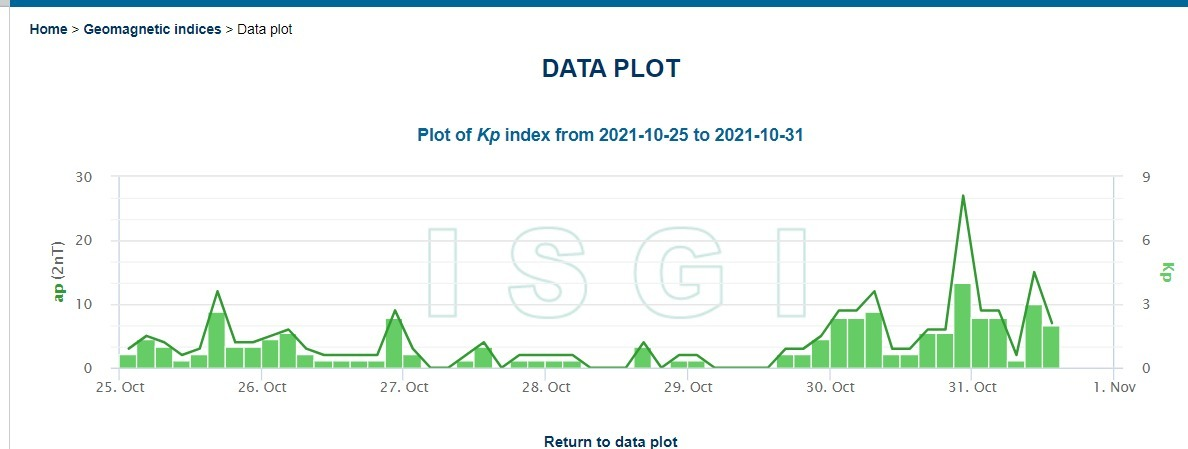
\includegraphics[width=1\textwidth,height=\textheight]{fig_src_isgi.png}
\caption{The source's provisional ISGI plot of Kp and ap, 25--31 October
2021 (definitive values in Table 4 and Figure 9).}
\end{figure}

\begin{figure}
\centering
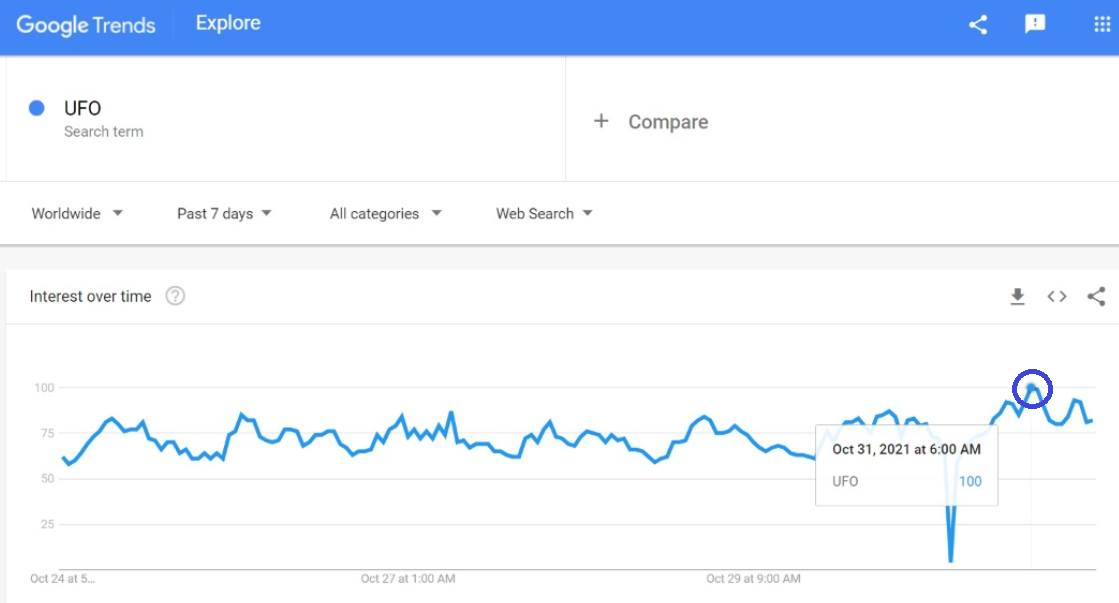
\includegraphics[width=1\textwidth,height=\textheight]{fig_src_trends7d.png}
\caption{The source's Google Trends screenshot: worldwide hourly search
interest in \emph{UFO} over the trailing seven days, with the maximum
circled and dated by the tooltip to 31 October 2021, 06:00 (observer
time, UTC+3).}
\end{figure}

\begin{figure}
\centering
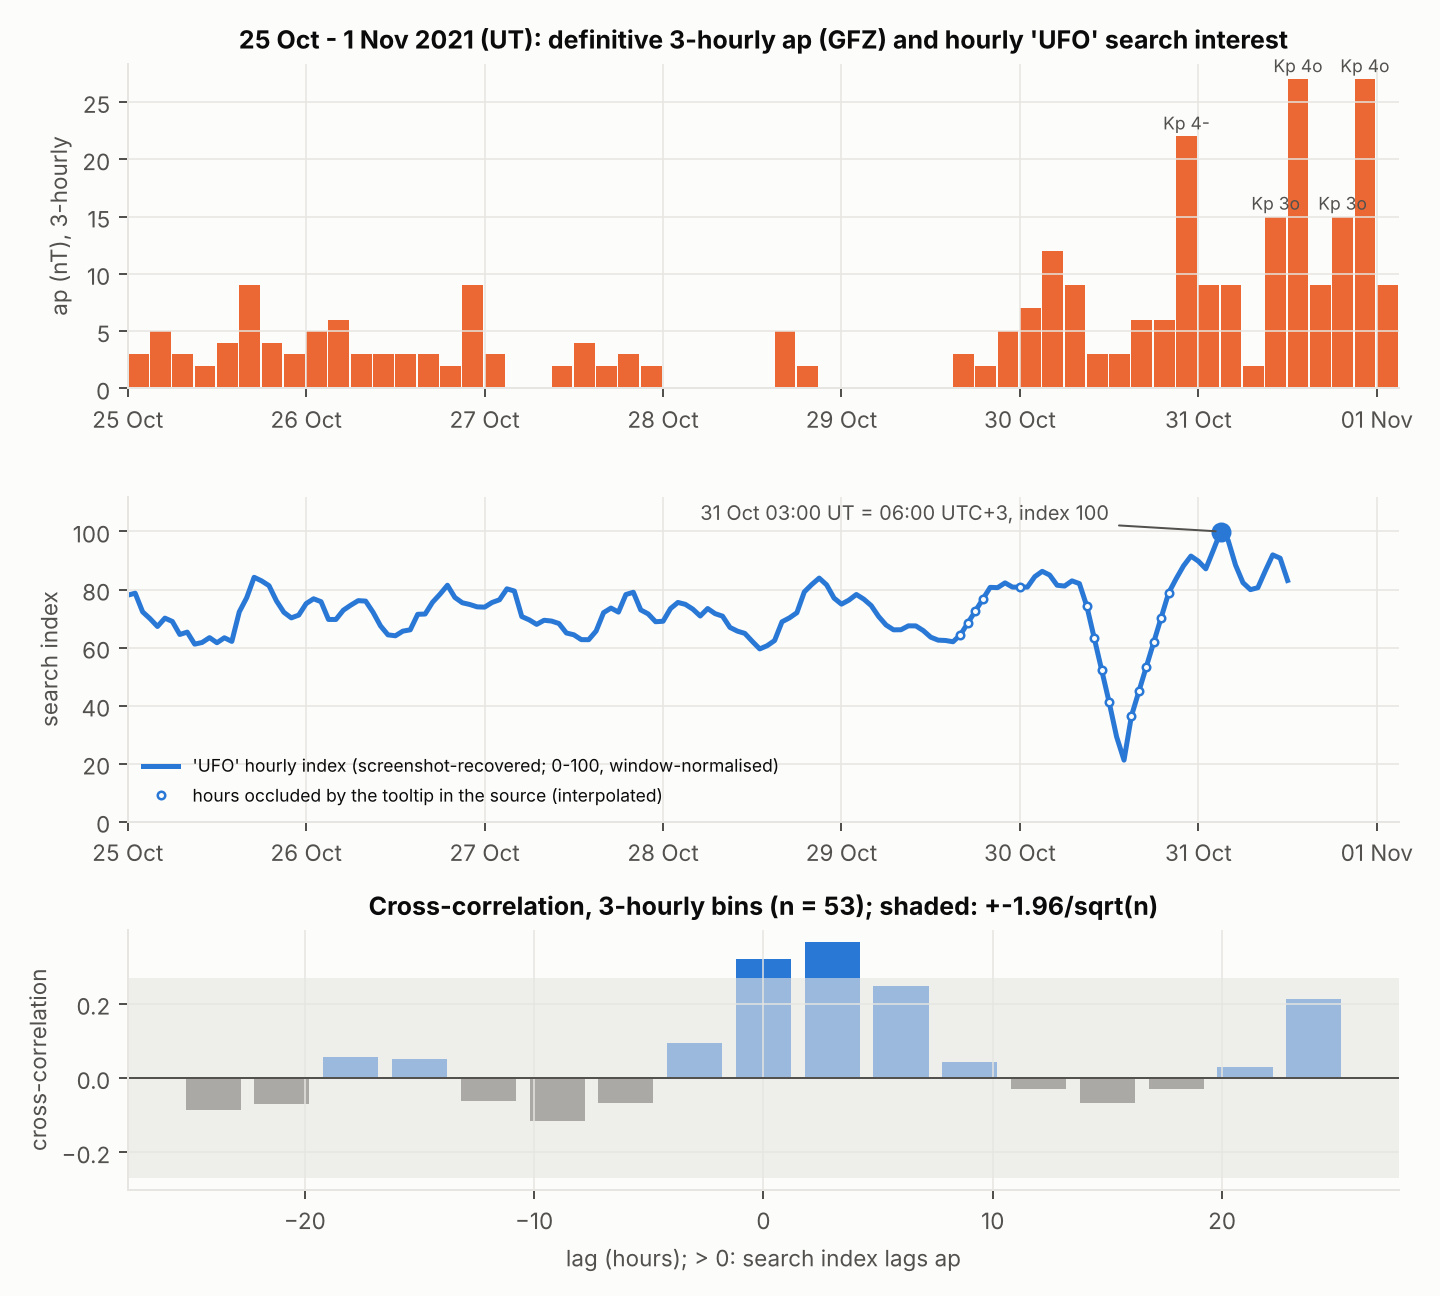
\includegraphics[width=1\textwidth,height=\textheight]{fig_S3_event.png}
\caption{Event window in Universal Time. Upper panel: definitive
three-hourly ap with the Bartels Kp steps of the five most disturbed
intervals. Middle panel: the recovered hourly search index; open markers
are the hours occluded by the tooltip in the source. Lower panel:
cross-correlation by lag on three-hour bins with the ±1.96/√n band.}
\end{figure}

\hypertarget{high-variance-anomalies-syria-and-albania}{%
\subsection{3.6 High-variance anomalies: Syria and
Albania}\label{high-variance-anomalies-syria-and-albania}}

In the source's ``interest by region'' panel for the same window, the
two jurisdictions with the highest normalised search propensity for
\emph{UFO} were Syria and Albania, far ahead of the rest. The source
connects the second with a rumour corpus of the 1990s concerning the
territory's role as a transshipment hub for human organs and narcotic
preparations, the first with contemporaneous reports of analogous flows
under conditions of armed conflict, and both with the long-standing
interest of the conventional visitor in acquiring human subjects for
non-consensual biometric sampling. We report the rumour as rumour and
verify none of it.

The statistical objection is the small-denominator effect: the regional
index is a share of all searches in the jurisdiction, so that in a
jurisdiction with few searches the share has a variance inversely
proportional to the total, and the extreme values of a normalised index
across some two hundred jurisdictions are expected to come from the
smallest denominators. The objection explains why the variance of the
two values is high. It does not explain why the high variance was
realised in those two jurisdictions rather than in any two of the
hundred or so with comparably small denominators, and the harvest
hypothesis, for what it is worth, predicts that search propensity is
maximal where affective amplitude is high (conflict, dislocation) and
where the logistics of biometric acquisition have a reported precedent.
Both conditions obtain in both jurisdictions. We lacked the regional
series and could not test the prediction. The anomaly is reported
without resolution, which is the condition in which the source left it.

\hypertarget{computational-protocol}{%
\subsection{3.7 Computational protocol}\label{computational-protocol}}

Everything reported above is produced by four scripts in the
supplementary archive: \texttt{parse\_sw.py} (definitive series),
\texttt{digitise.py} (figure recovery), \texttt{analysis.py} (all
statistics, written to \texttt{results.json}) and \texttt{figures.py}.
Listing 1 is the condensed core; it reproduces every headline number of
Sections 3.1--3.5 and the calibration of Section 2.4 from the three
intermediate files. If a Google Trends export of the vintage series
(\texttt{multiTimeline.csv}) is placed beside the scripts,
\texttt{analysis.py} replaces the digitised search component with a
model fit on the export and recomputes.

\begin{Shaded}
\begin{Highlighting}[]
\CommentTok{\#!/usr/bin/env python3}
\CommentTok{\# Listing 1. Reproducible core of Section 3 (condensed from analysis.py in the archive).}
\CommentTok{\# Inputs: kp\_ap\_daily.csv (parse\_sw.py); digitised\_components.csv and}
\CommentTok{\#         digitised\_trends7d.csv (digitise.py).}
\ImportTok{import}\NormalTok{ numpy }\ImportTok{as}\NormalTok{ np, pandas }\ImportTok{as}\NormalTok{ pd}
\ImportTok{from}\NormalTok{ scipy }\ImportTok{import}\NormalTok{ signal}
\ImportTok{from}\NormalTok{ prophet }\ImportTok{import}\NormalTok{ Prophet}
\ImportTok{from}\NormalTok{ statsmodels.tsa.api }\ImportTok{import}\NormalTok{ VAR}
\NormalTok{N, P, H }\OperatorTok{=} \DecValTok{10}\NormalTok{, }\FloatTok{365.0}\NormalTok{, }\DecValTok{303}          \CommentTok{\# Fourier order, grid period, 31 Oct (0{-}based day)}

\KeywordTok{def}\NormalTok{ fourier\_fit(y, n}\OperatorTok{=}\NormalTok{N):}
\NormalTok{    t }\OperatorTok{=}\NormalTok{ np.arange(}\BuiltInTok{len}\NormalTok{(y))}\OperatorTok{;}\NormalTok{ k }\OperatorTok{=}\NormalTok{ np.arange(}\DecValTok{1}\NormalTok{, n }\OperatorTok{+} \DecValTok{1}\NormalTok{)}
\NormalTok{    arg }\OperatorTok{=} \DecValTok{2} \OperatorTok{*}\NormalTok{ np.pi }\OperatorTok{*}\NormalTok{ np.outer(t, k) }\OperatorTok{/}\NormalTok{ P}
\NormalTok{    X }\OperatorTok{=}\NormalTok{ np.hstack([np.ones((}\BuiltInTok{len}\NormalTok{(y), }\DecValTok{1}\NormalTok{)), np.cos(arg), np.sin(arg)])}
\NormalTok{    b }\OperatorTok{=}\NormalTok{ np.linalg.lstsq(X, y, rcond}\OperatorTok{=}\VariableTok{None}\NormalTok{)[}\DecValTok{0}\NormalTok{]}\OperatorTok{;}\NormalTok{ fit }\OperatorTok{=}\NormalTok{ X }\OperatorTok{@}\NormalTok{ b}
\NormalTok{    r2 }\OperatorTok{=} \DecValTok{1} \OperatorTok{{-}}\NormalTok{ ((y }\OperatorTok{{-}}\NormalTok{ fit) }\OperatorTok{**} \DecValTok{2}\NormalTok{).}\BuiltInTok{sum}\NormalTok{() }\OperatorTok{/}\NormalTok{ ((y }\OperatorTok{{-}}\NormalTok{ y.mean()) }\OperatorTok{**} \DecValTok{2}\NormalTok{).}\BuiltInTok{sum}\NormalTok{()}
    \ControlFlowTok{return}\NormalTok{ np.hypot(b[}\DecValTok{1}\NormalTok{:n }\OperatorTok{+} \DecValTok{1}\NormalTok{], b[n }\OperatorTok{+} \DecValTok{1}\NormalTok{:]), np.arctan2(b[n }\OperatorTok{+} \DecValTok{1}\NormalTok{:], b[}\DecValTok{1}\NormalTok{:n }\OperatorTok{+} \DecValTok{1}\NormalTok{]), r2}

\KeywordTok{def}\NormalTok{ coherence(sU, sA, taus):      }\CommentTok{\# C(tau) = \textless{}sU(.+tau), sA(.)\textgreater{} / (|sU| |sA|), circular}
\NormalTok{    u, a }\OperatorTok{=}\NormalTok{ sU }\OperatorTok{{-}}\NormalTok{ sU.mean(), sA }\OperatorTok{{-}}\NormalTok{ sA.mean()}
\NormalTok{    d }\OperatorTok{=}\NormalTok{ np.linalg.norm(u) }\OperatorTok{*}\NormalTok{ np.linalg.norm(a)}
    \ControlFlowTok{return}\NormalTok{ np.array([np.dot(np.roll(u, }\OperatorTok{{-}}\NormalTok{t), a) }\OperatorTok{/}\NormalTok{ d }\ControlFlowTok{for}\NormalTok{ t }\KeywordTok{in}\NormalTok{ taus])}

\KeywordTok{def}\NormalTok{ phase(s):                     }\CommentTok{\# analytic{-}signal phase; exact on a full period}
    \ControlFlowTok{return}\NormalTok{ np.angle(signal.hilbert(s }\OperatorTok{{-}}\NormalTok{ s.mean()))}

\KeywordTok{def}\NormalTok{ rayleigh(th):}
\NormalTok{    n }\OperatorTok{=} \BuiltInTok{len}\NormalTok{(th)}\OperatorTok{;}\NormalTok{ Rb }\OperatorTok{=} \BuiltInTok{abs}\NormalTok{(np.exp(}\OtherTok{1j} \OperatorTok{*}\NormalTok{ np.asarray(th)).mean())}\OperatorTok{;}\NormalTok{ Z }\OperatorTok{=}\NormalTok{ n }\OperatorTok{*}\NormalTok{ Rb }\OperatorTok{**} \DecValTok{2}
\NormalTok{    p }\OperatorTok{=}\NormalTok{ np.exp(}\OperatorTok{{-}}\NormalTok{Z) }\OperatorTok{*}\NormalTok{ (}\DecValTok{1} \OperatorTok{+}\NormalTok{ (}\DecValTok{2} \OperatorTok{*}\NormalTok{ Z }\OperatorTok{{-}}\NormalTok{ Z }\OperatorTok{**} \DecValTok{2}\NormalTok{) }\OperatorTok{/}\NormalTok{ (}\DecValTok{4} \OperatorTok{*}\NormalTok{ n)}
                      \OperatorTok{{-}}\NormalTok{ (}\DecValTok{24} \OperatorTok{*}\NormalTok{ Z }\OperatorTok{{-}} \DecValTok{132} \OperatorTok{*}\NormalTok{ Z }\OperatorTok{**} \DecValTok{2} \OperatorTok{+} \DecValTok{76} \OperatorTok{*}\NormalTok{ Z }\OperatorTok{**} \DecValTok{3} \OperatorTok{{-}} \DecValTok{9} \OperatorTok{*}\NormalTok{ Z }\OperatorTok{**} \DecValTok{4}\NormalTok{) }\OperatorTok{/}\NormalTok{ (}\DecValTok{288} \OperatorTok{*}\NormalTok{ n }\OperatorTok{**} \DecValTok{2}\NormalTok{))}
    \ControlFlowTok{return}\NormalTok{ Rb, Z, p}

\KeywordTok{def}\NormalTok{ peaks(s, frac}\OperatorTok{=}\FloatTok{0.10}\NormalTok{):}
\NormalTok{    e }\OperatorTok{=}\NormalTok{ np.concatenate([s, s, s])}
\NormalTok{    p, \_ }\OperatorTok{=}\NormalTok{ signal.find\_peaks(e, prominence}\OperatorTok{=}\NormalTok{frac }\OperatorTok{*}\NormalTok{ np.ptp(s))}
    \ControlFlowTok{return}\NormalTok{ np.unique(p[(p }\OperatorTok{\textgreater{}=} \BuiltInTok{len}\NormalTok{(s)) }\OperatorTok{\&}\NormalTok{ (p }\OperatorTok{\textless{}} \DecValTok{2} \OperatorTok{*} \BuiltInTok{len}\NormalTok{(s))] }\OperatorTok{{-}} \BuiltInTok{len}\NormalTok{(s))}

\KeywordTok{def}\NormalTok{ prophet\_yearly(series):       }\CommentTok{\# Prophet, multiplicative, yearly order 10, \% of trend}
\NormalTok{    df }\OperatorTok{=}\NormalTok{ pd.DataFrame(\{}\StringTok{"ds"}\NormalTok{: series.index, }\StringTok{"y"}\NormalTok{: series.values\})}
\NormalTok{    m }\OperatorTok{=}\NormalTok{ Prophet(yearly\_seasonality}\OperatorTok{=}\NormalTok{N, weekly\_seasonality}\OperatorTok{=}\VariableTok{False}\NormalTok{,}
\NormalTok{                daily\_seasonality}\OperatorTok{=}\VariableTok{False}\NormalTok{, seasonality\_mode}\OperatorTok{=}\StringTok{"multiplicative"}\NormalTok{).fit(df)}
\NormalTok{    grid }\OperatorTok{=}\NormalTok{ pd.DataFrame(\{}\StringTok{"ds"}\NormalTok{: pd.date\_range(}\StringTok{"2017{-}01{-}01"}\NormalTok{, periods}\OperatorTok{=}\DecValTok{365}\NormalTok{)\})}
    \ControlFlowTok{return} \DecValTok{100} \OperatorTok{*}\NormalTok{ m.predict(grid)[}\StringTok{"yearly"}\NormalTok{].values}

\NormalTok{kp }\OperatorTok{=}\NormalTok{ pd.read\_csv(}\StringTok{"kp\_ap\_daily.csv"}\NormalTok{, index\_col}\OperatorTok{=}\DecValTok{0}\NormalTok{, parse\_dates}\OperatorTok{=}\VariableTok{True}\NormalTok{)}
\NormalTok{comp }\OperatorTok{=}\NormalTok{ pd.read\_csv(}\StringTok{"digitised\_components.csv"}\NormalTok{, index\_col}\OperatorTok{=}\DecValTok{0}\NormalTok{)}
\NormalTok{tr7 }\OperatorTok{=}\NormalTok{ pd.read\_csv(}\StringTok{"digitised\_trends7d.csv"}\NormalTok{, index\_col}\OperatorTok{=}\DecValTok{0}\NormalTok{, parse\_dates}\OperatorTok{=}\VariableTok{True}\NormalTok{)}

\CommentTok{\# {-}{-}{-} 3.1  recompute the Ap component on the definitive series; validate the digitisation}
\NormalTok{sA\_def }\OperatorTok{=}\NormalTok{ prophet\_yearly(kp.loc[}\StringTok{"2004{-}01{-}01"}\NormalTok{:}\StringTok{"2021{-}09{-}30"}\NormalTok{, }\StringTok{"Ap"}\NormalTok{].astype(}\BuiltInTok{float}\NormalTok{))}
\BuiltInTok{print}\NormalTok{(}\StringTok{"r(definitive, fig4 / fig5 Ap) ="}\NormalTok{,}
\NormalTok{      np.corrcoef(sA\_def, comp[}\StringTok{"fig4\_Ap"}\NormalTok{])[}\DecValTok{0}\NormalTok{, }\DecValTok{1}\NormalTok{].}\BuiltInTok{round}\NormalTok{(}\DecValTok{3}\NormalTok{),}
\NormalTok{      np.corrcoef(sA\_def, comp[}\StringTok{"fig5\_Ap"}\NormalTok{])[}\DecValTok{0}\NormalTok{, }\DecValTok{1}\NormalTok{].}\BuiltInTok{round}\NormalTok{(}\DecValTok{3}\NormalTok{))}
\BuiltInTok{print}\NormalTok{(}\StringTok{"definitive Ap component, 31 Oct: }\SpecialCharTok{\%.1f\%\%}\StringTok{, rank }\SpecialCharTok{\%d}\StringTok{/365; maxima at DOY }\SpecialCharTok{\%s}\StringTok{"}
      \OperatorTok{\%}\NormalTok{ (sA\_def[H], (sA\_def }\OperatorTok{\textgreater{}}\NormalTok{ sA\_def[H]).}\BuiltInTok{sum}\NormalTok{() }\OperatorTok{+} \DecValTok{1}\NormalTok{, peaks(sA\_def)))}

\CommentTok{\# {-}{-}{-} 3.3 / 3.4  coherence, harmonic phases, instantaneous phase, peak pairing}
\NormalTok{taus }\OperatorTok{=}\NormalTok{ np.arange(}\OperatorTok{{-}}\DecValTok{90}\NormalTok{, }\DecValTok{91}\NormalTok{)}
\ControlFlowTok{for}\NormalTok{ fig }\KeywordTok{in}\NormalTok{ (}\StringTok{"fig4"}\NormalTok{, }\StringTok{"fig5"}\NormalTok{):}
\NormalTok{    sU, sA }\OperatorTok{=}\NormalTok{ comp[}\SpecialStringTok{f"}\SpecialCharTok{\{}\NormalTok{fig}\SpecialCharTok{\}}\SpecialStringTok{\_UFO"}\NormalTok{].values, comp[}\SpecialStringTok{f"}\SpecialCharTok{\{}\NormalTok{fig}\SpecialCharTok{\}}\SpecialStringTok{\_Ap"}\NormalTok{].values}
\NormalTok{    C }\OperatorTok{=}\NormalTok{ coherence(sU, sA, taus)}\OperatorTok{;}\NormalTok{ i }\OperatorTok{=}\NormalTok{ C.argmin()}
\NormalTok{    AU, phU, r2U }\OperatorTok{=}\NormalTok{ fourier\_fit(sU)}\OperatorTok{;}\NormalTok{ AA, phA, r2A }\OperatorTok{=}\NormalTok{ fourier\_fit(sA)}
\NormalTok{    dphi }\OperatorTok{=}\NormalTok{ np.degrees(np.angle(np.exp(}\OtherTok{1j} \OperatorTok{*}\NormalTok{ (phU }\OperatorTok{{-}}\NormalTok{ phA))))}
\NormalTok{    pA, pU }\OperatorTok{=}\NormalTok{ peaks(sA), peaks(sU)}\OperatorTok{;}\NormalTok{ lags }\OperatorTok{=}\NormalTok{ []}
    \ControlFlowTok{for}\NormalTok{ p }\KeywordTok{in}\NormalTok{ pA:                  }\CommentTok{\# first UFO maximum within 45 d after each Ap maximum}
\NormalTok{        l }\OperatorTok{=}\NormalTok{ (pU }\OperatorTok{{-}}\NormalTok{ p) }\OperatorTok{\%} \DecValTok{365}\OperatorTok{;}\NormalTok{ l }\OperatorTok{=}\NormalTok{ l[(l }\OperatorTok{\textgreater{}} \DecValTok{0}\NormalTok{) }\OperatorTok{\&}\NormalTok{ (l }\OperatorTok{\textless{}=} \DecValTok{45}\NormalTok{)]}
        \ControlFlowTok{if} \BuiltInTok{len}\NormalTok{(l): lags.append(l.}\BuiltInTok{min}\NormalTok{())}
\NormalTok{    Rb, Z, pr }\OperatorTok{=}\NormalTok{ rayleigh(}\DecValTok{2} \OperatorTok{*}\NormalTok{ np.pi }\OperatorTok{*}\NormalTok{ np.array(lags) }\OperatorTok{/}\NormalTok{ (P }\OperatorTok{/}\NormalTok{ N))}
\NormalTok{    d0 }\OperatorTok{=}\NormalTok{ phase(sU) }\OperatorTok{{-}}\NormalTok{ phase(sA)}
    \BuiltInTok{print}\NormalTok{(}\SpecialStringTok{f"}\SpecialCharTok{\{}\NormalTok{fig}\SpecialCharTok{\}}\SpecialStringTok{: R2 }\SpecialCharTok{\{}\NormalTok{r2U}\SpecialCharTok{:.4f\}}\SpecialStringTok{/}\SpecialCharTok{\{}\NormalTok{r2A}\SpecialCharTok{:.4f\}}\SpecialStringTok{ | C(0) }\SpecialCharTok{\{}\NormalTok{C[taus }\OperatorTok{==} \DecValTok{0}\NormalTok{][}\DecValTok{0}\NormalTok{]}\SpecialCharTok{:+.2f\}}\SpecialStringTok{ | "}
          \SpecialStringTok{f"min C }\SpecialCharTok{\{}\NormalTok{C[i]}\SpecialCharTok{:+.2f\}}\SpecialStringTok{ at tau }\SpecialCharTok{\{}\NormalTok{taus[i]}\SpecialCharTok{:+d\}}\SpecialStringTok{ d | dphi(n=2) }\SpecialCharTok{\{}\NormalTok{dphi[}\DecValTok{1}\NormalTok{]}\SpecialCharTok{:+.0f\}}\SpecialStringTok{ deg | "}
          \SpecialStringTok{f"PLV(0) }\SpecialCharTok{\{}\BuiltInTok{abs}\NormalTok{(np.exp(}\OtherTok{1j} \OperatorTok{*}\NormalTok{ d0).mean())}\SpecialCharTok{:.2f\}}\SpecialStringTok{, "}
          \SpecialStringTok{f"mean dphi }\SpecialCharTok{\{}\NormalTok{np}\SpecialCharTok{.}\NormalTok{degrees(np.angle(np.exp(}\OtherTok{1j} \OperatorTok{*}\NormalTok{ d0).mean()))}\SpecialCharTok{:+.0f\}}\SpecialStringTok{ deg | "}
          \SpecialStringTok{f"pairs }\SpecialCharTok{\{}\BuiltInTok{len}\NormalTok{(lags)}\SpecialCharTok{\}}\SpecialStringTok{/}\SpecialCharTok{\{}\BuiltInTok{len}\NormalTok{(pA)}\SpecialCharTok{\}}\SpecialStringTok{, lag }\SpecialCharTok{\{}\NormalTok{np}\SpecialCharTok{.}\NormalTok{mean(lags)}\SpecialCharTok{:.1f\}}\SpecialStringTok{ +{-} "}
          \SpecialStringTok{f"}\SpecialCharTok{\{}\NormalTok{np}\SpecialCharTok{.}\NormalTok{std(lags, ddof}\OperatorTok{=}\DecValTok{1}\NormalTok{)}\SpecialCharTok{:.1f\}}\SpecialStringTok{ d, Rayleigh p }\SpecialCharTok{\{}\NormalTok{pr}\SpecialCharTok{:.2f\}}\SpecialStringTok{ | "}
          \SpecialStringTok{f"Ap max nearest 31 Oct: DOY }\SpecialCharTok{\{}\NormalTok{pA[np.argmin(np.}\BuiltInTok{abs}\NormalTok{((pA }\OperatorTok{{-}}\NormalTok{ H }\OperatorTok{+} \DecValTok{182}\NormalTok{) }\OperatorTok{\%} \DecValTok{365} \OperatorTok{{-}} \DecValTok{182}\NormalTok{))]}\SpecialCharTok{\}}\SpecialStringTok{"}\NormalTok{)}

\CommentTok{\# {-}{-}{-} 3.2  climatology of Ap on the festival}
\KeywordTok{def}\NormalTok{ clim(df):}
\NormalTok{    d }\OperatorTok{=}\NormalTok{ df.index.dayofyear.values }\OperatorTok{{-}} \DecValTok{1}
\NormalTok{    d }\OperatorTok{=}\NormalTok{ np.where(np.asarray(df.index.is\_leap\_year) }\OperatorTok{\&}\NormalTok{ (d }\OperatorTok{\textgreater{}=} \DecValTok{59}\NormalTok{), d }\OperatorTok{{-}} \DecValTok{1}\NormalTok{, d)}
    \ControlFlowTok{return}\NormalTok{ df[}\StringTok{"Ap"}\NormalTok{].groupby(d).mean().reindex(}\BuiltInTok{range}\NormalTok{(}\DecValTok{365}\NormalTok{)).values}
\NormalTok{windows }\OperatorTok{=}\NormalTok{ ((}\StringTok{"2004{-}2021"}\NormalTok{, kp.loc[}\StringTok{"2004{-}01{-}01"}\NormalTok{:}\StringTok{"2021{-}09{-}30"}\NormalTok{]), (}\StringTok{"1957{-}2025"}\NormalTok{, kp),}
\NormalTok{           (}\StringTok{"excl. 2003"}\NormalTok{, kp[kp.index.year }\OperatorTok{!=} \DecValTok{2003}\NormalTok{]))}
\ControlFlowTok{for}\NormalTok{ lab, df }\KeywordTok{in}\NormalTok{ windows:}
\NormalTok{    c }\OperatorTok{=}\NormalTok{ clim(df)}\OperatorTok{;}\NormalTok{ rng }\OperatorTok{=}\NormalTok{ np.random.default\_rng(}\DecValTok{0}\NormalTok{)}
\NormalTok{    w }\OperatorTok{=} \KeywordTok{lambda}\NormalTok{ s: np.mean([c[(s }\OperatorTok{+}\NormalTok{ k) }\OperatorTok{\%} \DecValTok{365}\NormalTok{] }\ControlFlowTok{for}\NormalTok{ k }\KeywordTok{in} \BuiltInTok{range}\NormalTok{(}\OperatorTok{{-}}\DecValTok{2}\NormalTok{, }\DecValTok{3}\NormalTok{)])}
\NormalTok{    pW }\OperatorTok{=}\NormalTok{ np.mean([w(s) }\OperatorTok{\textgreater{}=}\NormalTok{ w(H) }\ControlFlowTok{for}\NormalTok{ s }\KeywordTok{in}\NormalTok{ rng.integers(}\DecValTok{0}\NormalTok{, }\DecValTok{365}\NormalTok{, }\DecValTok{20000}\NormalTok{)])}
    \BuiltInTok{print}\NormalTok{(}\SpecialStringTok{f"climatology }\SpecialCharTok{\{}\NormalTok{lab}\SpecialCharTok{\}}\SpecialStringTok{: Ap(31 Oct) }\SpecialCharTok{\{}\NormalTok{c[H]}\SpecialCharTok{:.1f\}}\SpecialStringTok{ vs mean }\SpecialCharTok{\{}\NormalTok{df[}\StringTok{\textquotesingle{}Ap\textquotesingle{}}\NormalTok{]}\SpecialCharTok{.}\NormalTok{mean()}\SpecialCharTok{:.1f\}}\SpecialStringTok{, "}
          \SpecialStringTok{f"percentile }\SpecialCharTok{\{}\DecValTok{100} \OperatorTok{*}\NormalTok{ (c }\OperatorTok{\textless{}}\NormalTok{ c[H])}\SpecialCharTok{.}\NormalTok{mean()}\SpecialCharTok{:.0f\}}\SpecialStringTok{, window 29 Oct{-}2 Nov perm. p }\SpecialCharTok{\{}\NormalTok{pW}\SpecialCharTok{:.3f\}}\SpecialStringTok{"}\NormalTok{)}

\CommentTok{\# {-}{-}{-} 3.5  event window: 3{-}hourly ap (UT) against the hourly search index (UTC+3 {-}\textgreater{} UT)}
\NormalTok{ev }\OperatorTok{=}\NormalTok{ kp.loc[}\StringTok{"2021{-}10{-}25"}\NormalTok{:}\StringTok{"2021{-}11{-}01"}\NormalTok{]}\OperatorTok{;}\NormalTok{ rows }\OperatorTok{=}\NormalTok{ []}
\ControlFlowTok{for}\NormalTok{ d, r }\KeywordTok{in}\NormalTok{ ev.iterrows():}
\NormalTok{    rows }\OperatorTok{+=}\NormalTok{ [}\BuiltInTok{dict}\NormalTok{(t}\OperatorTok{=}\NormalTok{d }\OperatorTok{+}\NormalTok{ pd.Timedelta(hours}\OperatorTok{=}\DecValTok{3} \OperatorTok{*}\NormalTok{ i), ap}\OperatorTok{=}\NormalTok{r[}\SpecialStringTok{f"ap}\SpecialCharTok{\{}\NormalTok{i}\SpecialCharTok{\}}\SpecialStringTok{"}\NormalTok{], Kp10}\OperatorTok{=}\NormalTok{r[}\SpecialStringTok{f"Kp}\SpecialCharTok{\{}\NormalTok{i}\SpecialCharTok{\}}\SpecialStringTok{"}\NormalTok{])}
             \ControlFlowTok{for}\NormalTok{ i }\KeywordTok{in} \BuiltInTok{range}\NormalTok{(}\DecValTok{8}\NormalTok{)]}
\NormalTok{tab }\OperatorTok{=}\NormalTok{ pd.DataFrame(rows).set\_index(}\StringTok{"t"}\NormalTok{)}
\NormalTok{u }\OperatorTok{=}\NormalTok{ tr7[}\StringTok{"ufo\_hourly"}\NormalTok{].copy()}\OperatorTok{;}\NormalTok{ u.index }\OperatorTok{=}\NormalTok{ u.index }\OperatorTok{{-}}\NormalTok{ pd.Timedelta(hours}\OperatorTok{=}\DecValTok{3}\NormalTok{)}
\NormalTok{both }\OperatorTok{=}\NormalTok{ pd.concat([tab[}\StringTok{"ap"}\NormalTok{], u.resample(}\StringTok{"3h"}\NormalTok{).mean().rename(}\StringTok{"ufo"}\NormalTok{)], axis}\OperatorTok{=}\DecValTok{1}\NormalTok{,}
\NormalTok{                 sort}\OperatorTok{=}\VariableTok{True}\NormalTok{).dropna()}
\NormalTok{x }\OperatorTok{=}\NormalTok{ np.log1p(both[}\StringTok{"ap"}\NormalTok{].values)}\OperatorTok{;}\NormalTok{ y }\OperatorTok{=}\NormalTok{ both[}\StringTok{"ufo"}\NormalTok{].values}
\NormalTok{x }\OperatorTok{=}\NormalTok{ (x }\OperatorTok{{-}}\NormalTok{ x.mean()) }\OperatorTok{/}\NormalTok{ x.std()}\OperatorTok{;}\NormalTok{ y }\OperatorTok{=}\NormalTok{ (y }\OperatorTok{{-}}\NormalTok{ y.mean()) }\OperatorTok{/}\NormalTok{ y.std()}
\NormalTok{cc }\OperatorTok{=}\NormalTok{ \{l: (np.mean(x[:}\BuiltInTok{len}\NormalTok{(x) }\OperatorTok{{-}}\NormalTok{ l] }\OperatorTok{*}\NormalTok{ y[l:]) }\ControlFlowTok{if}\NormalTok{ l }\OperatorTok{\textgreater{}=} \DecValTok{0} \ControlFlowTok{else}\NormalTok{ np.mean(x[}\OperatorTok{{-}}\NormalTok{l:] }\OperatorTok{*}\NormalTok{ y[:}\BuiltInTok{len}\NormalTok{(y) }\OperatorTok{+}\NormalTok{ l]))}
      \ControlFlowTok{for}\NormalTok{ l }\KeywordTok{in} \BuiltInTok{range}\NormalTok{(}\OperatorTok{{-}}\DecValTok{8}\NormalTok{, }\DecValTok{9}\NormalTok{)\}}
\BuiltInTok{print}\NormalTok{(}\StringTok{"search max (UT):"}\NormalTok{, u.idxmax(), }\StringTok{"| CCF max at lag"}\NormalTok{, }\DecValTok{3} \OperatorTok{*} \BuiltInTok{max}\NormalTok{(cc, key}\OperatorTok{=}\NormalTok{cc.get),}
      \StringTok{"h, r ="}\NormalTok{, }\BuiltInTok{round}\NormalTok{(}\BuiltInTok{max}\NormalTok{(cc.values()), }\DecValTok{3}\NormalTok{), }\StringTok{"| noise"}\NormalTok{, }\BuiltInTok{round}\NormalTok{(}\FloatTok{1.96} \OperatorTok{/}\NormalTok{ np.sqrt(}\BuiltInTok{len}\NormalTok{(x)), }\DecValTok{3}\NormalTok{))}
\NormalTok{data }\OperatorTok{=}\NormalTok{ pd.DataFrame(\{}\StringTok{"ap"}\NormalTok{: np.log1p(both[}\StringTok{"ap"}\NormalTok{].values), }\StringTok{"ufo"}\NormalTok{: both[}\StringTok{"ufo"}\NormalTok{].values\},}
\NormalTok{                    index}\OperatorTok{=}\NormalTok{both.index)}
\NormalTok{p }\OperatorTok{=} \BuiltInTok{max}\NormalTok{(}\BuiltInTok{int}\NormalTok{(VAR(data).select\_order(}\DecValTok{4}\NormalTok{).bic), }\DecValTok{1}\NormalTok{)}\OperatorTok{;}\NormalTok{ res }\OperatorTok{=}\NormalTok{ VAR(data).fit(p)}
\BuiltInTok{print}\NormalTok{(}\SpecialStringTok{f"VAR(}\SpecialCharTok{\{}\NormalTok{p}\SpecialCharTok{\}}\SpecialStringTok{): Granger ap{-}\textgreater{}ufo p = "}
      \SpecialStringTok{f"}\SpecialCharTok{\{}\NormalTok{res}\SpecialCharTok{.}\NormalTok{test\_causality(}\StringTok{\textquotesingle{}ufo\textquotesingle{}}\NormalTok{, [}\StringTok{\textquotesingle{}ap\textquotesingle{}}\NormalTok{], kind}\OperatorTok{=}\StringTok{\textquotesingle{}f\textquotesingle{}}\NormalTok{)}\SpecialCharTok{.}\NormalTok{pvalue}\SpecialCharTok{:.3f\}}\SpecialStringTok{; ufo{-}\textgreater{}ap p = "}
      \SpecialStringTok{f"}\SpecialCharTok{\{}\NormalTok{res}\SpecialCharTok{.}\NormalTok{test\_causality(}\StringTok{\textquotesingle{}ap\textquotesingle{}}\NormalTok{, [}\StringTok{\textquotesingle{}ufo\textquotesingle{}}\NormalTok{], kind}\OperatorTok{=}\StringTok{\textquotesingle{}f\textquotesingle{}}\NormalTok{)}\SpecialCharTok{.}\NormalTok{pvalue}\SpecialCharTok{:.3f\}}\SpecialStringTok{; "}
      \SpecialStringTok{f"IRF peak at }\SpecialCharTok{\{}\DecValTok{3} \OperatorTok{*} \BuiltInTok{int}\NormalTok{(np.argmax(res.irf(}\DecValTok{8}\NormalTok{).irfs[:, }\DecValTok{1}\NormalTok{, }\DecValTok{0}\NormalTok{]))}\SpecialCharTok{\}}\SpecialStringTok{ h"}\NormalTok{)}

\CommentTok{\# {-}{-}{-} Section 2 calibration: Kuramoto ensemble whose coupling is driven by the field}
\NormalTok{rng }\OperatorTok{=}\NormalTok{ np.random.default\_rng(}\DecValTok{1}\NormalTok{)}\OperatorTok{;}\NormalTok{ n, sig, K0, dt }\OperatorTok{=} \DecValTok{400}\NormalTok{, }\FloatTok{0.5}\NormalTok{, }\FloatTok{0.5}\NormalTok{, }\FloatTok{0.05}
\NormalTok{om, th }\OperatorTok{=}\NormalTok{ rng.normal(}\DecValTok{0}\NormalTok{, sig, n), rng.uniform(}\OperatorTok{{-}}\NormalTok{np.pi, np.pi, n)}
\NormalTok{apv }\OperatorTok{=}\NormalTok{ np.repeat(tab[}\StringTok{"ap"}\NormalTok{].values, }\BuiltInTok{int}\NormalTok{(}\DecValTok{3} \OperatorTok{/}\NormalTok{ dt))}\OperatorTok{;}\NormalTok{ r }\OperatorTok{=}\NormalTok{ []}
\ControlFlowTok{for}\NormalTok{ a }\KeywordTok{in}\NormalTok{ apv:                     }\CommentTok{\# K(t) = K0 + ap(t)/27 ; mean{-}field Kuramoto step}
\NormalTok{    z }\OperatorTok{=}\NormalTok{ np.exp(}\OtherTok{1j} \OperatorTok{*}\NormalTok{ th).mean()}\OperatorTok{;}\NormalTok{ r.append(}\BuiltInTok{abs}\NormalTok{(z))}
\NormalTok{    th }\OperatorTok{=}\NormalTok{ th }\OperatorTok{+}\NormalTok{ dt }\OperatorTok{*}\NormalTok{ (om }\OperatorTok{+}\NormalTok{ (K0 }\OperatorTok{+}\NormalTok{ a }\OperatorTok{/} \DecValTok{27}\NormalTok{) }\OperatorTok{*} \BuiltInTok{abs}\NormalTok{(z) }\OperatorTok{*}\NormalTok{ np.sin(np.angle(z) }\OperatorTok{{-}}\NormalTok{ th))}
\NormalTok{r }\OperatorTok{=}\NormalTok{ np.array(r)}\OperatorTok{;}\NormalTok{ Kc }\OperatorTok{=}\NormalTok{ sig }\OperatorTok{*}\NormalTok{ np.sqrt(}\DecValTok{8} \OperatorTok{/}\NormalTok{ np.pi)}
\BuiltInTok{print}\NormalTok{(}\SpecialStringTok{f"Kuramoto: Kc = }\SpecialCharTok{\{}\NormalTok{Kc}\SpecialCharTok{:.2f\}}\SpecialStringTok{ (crossed at ap = }\SpecialCharTok{\{}\NormalTok{(Kc }\OperatorTok{{-}}\NormalTok{ K0) }\OperatorTok{*} \DecValTok{27}\SpecialCharTok{:.1f\}}\SpecialStringTok{ nT); "}
      \SpecialStringTok{f"r 25{-}29 Oct }\SpecialCharTok{\{}\NormalTok{r[:}\BuiltInTok{int}\NormalTok{(}\DecValTok{120} \OperatorTok{/}\NormalTok{ dt)]}\SpecialCharTok{.}\NormalTok{mean()}\SpecialCharTok{:.2f\}}\SpecialStringTok{, r 31 Oct "}
      \SpecialStringTok{f"}\SpecialCharTok{\{}\NormalTok{r[}\BuiltInTok{int}\NormalTok{(}\DecValTok{144} \OperatorTok{/}\NormalTok{ dt):}\BuiltInTok{int}\NormalTok{(}\DecValTok{168} \OperatorTok{/}\NormalTok{ dt)]}\SpecialCharTok{.}\NormalTok{mean()}\SpecialCharTok{:.2f\}}\SpecialStringTok{, first r \textgreater{} 0.5 at "}
      \SpecialStringTok{f"}\SpecialCharTok{\{}\NormalTok{tab}\SpecialCharTok{.}\NormalTok{index[}\DecValTok{0}\NormalTok{] }\OperatorTok{+}\NormalTok{ pd}\SpecialCharTok{.}\NormalTok{Timedelta(hours}\OperatorTok{=}\BuiltInTok{float}\NormalTok{(np.argmax(r }\OperatorTok{\textgreater{}} \FloatTok{0.5}\NormalTok{) }\OperatorTok{*}\NormalTok{ dt))}\SpecialCharTok{\}}\SpecialStringTok{ UT"}\NormalTok{)}
\end{Highlighting}
\end{Shaded}

Output of Listing 1 on the archived inputs:

\begin{verbatim}
r(definitive, fig4 / fig5 Ap) = 0.99 0.952
definitive Ap component, 31 Oct: 5.3%, rank 125/365; maxima at DOY [ 22  64 162 203 246 312 354]
fig4: R2 0.9979/0.9977 | C(0) -0.29 | min C -0.49 at tau +15 d | dphi(n=2) -160 deg |
      PLV(0) 0.45, mean dphi +158 deg | pairs 6/8, lag 21.2 +- 13.6 d, Rayleigh p 0.63 |
      Ap max nearest 31 Oct: DOY 313
fig5: R2 1.0000/0.9992 | C(0) -0.23 | min C -0.56 at tau +12 d | dphi(n=2) -166 deg |
      PLV(0) 0.40, mean dphi +162 deg | pairs 7/8, lag 26.9 +- 13.0 d, Rayleigh p 0.18 |
      Ap max nearest 31 Oct: DOY 311
climatology 2004-2021: Ap(31 Oct) 6.2 vs mean 8.3, percentile 17, window 29 Oct-2 Nov perm. p 0.821
climatology 1957-2025: Ap(31 Oct) 15.3 vs mean 12.8, percentile 88, window 29 Oct-2 Nov perm. p 0.040
climatology excl. 2003: Ap(31 Oct) 13.8 vs mean 12.7, percentile 70, window 29 Oct-2 Nov perm. p 0.139
search max (UT): 2021-10-31 03:00:00 | CCF max at lag 3 h, r = 0.367 | noise 0.269
VAR(1): Granger ap->ufo p = 0.060; ufo->ap p = 0.278; IRF peak at 6 h
Kuramoto: Kc = 0.80 (crossed at ap = 8.0 nT); r 25-29 Oct 0.12, r 31 Oct 0.72,
          first r > 0.5 at 2021-10-30 23:03:00 UT
\end{verbatim}

\emph{Data and code availability.} Definitive indices: GFZ Potsdam via
the CSSI compilation at https://celestrak.org/SpaceData/ (no licence
restriction; attribution requested). Real-time indices: ISGI,
http://isgi.unistra.fr/data\_plot.php. The source's seven-day search
export:
https://docs.google.com/spreadsheets/d/1mZXsON8G8e5frev0sSoGPS\_hdJBtb1ZGglrbJ1\_xHSE.
Scripts, intermediate files, \texttt{results.json} and all figures:
supplementary archive.

\hypertarget{section-4.-conclusion-and-statement-of-concern}{%
\section{Section 4. Conclusion and Statement of
Concern}\label{section-4.-conclusion-and-statement-of-concern}}

\hypertarget{findings}{%
\subsection{4.1 Findings}\label{findings}}

H0 is rejected on the annual components and on the event week, in both
cases against the direction the source expected. The two annual
components are not independent; they are locked in opposition, with the
search curve the negative of the geomagnetic curve delayed by a
fortnight (\(C = -0.49\) to \(-0.57\) at \(\tau = 12\)--\(15\) d; mean
phase difference \(158°\)--\(162°\)), and the opposition is carried by
the semiannual harmonic, the only harmonic of the Hyperborean perimeter
whose phase returns from year to year. H1 survives in its lagged form
and dies in its simultaneous form: there is no positive alignment at two
to three weeks (\(C \le 0.17\)), the hand-drawn pairing of the source
reduces by rule to six or seven pairs whose lags are indistinguishable
from uniform scatter (\(p = 0.18\)--\(0.63\)), and the festival itself
is not a geomagnetic maximum but the flank of one that falls on 8--10
November, in a window in which the festival is a quiet date (17th
percentile) and is an active one only when the storms of 2003 are
admitted. Within the week of 2021 the order the source asserted is
observed: the field rose fourteen-fold into the festival, the search
maximum followed the first \(K_p\,4-\) interval by 4.5 h, the
cross-correlation peaks at \(+2\) to \(+3\) h above its noise level, and
the field Granger-causes the search index at \(p = 0.060\) while the
index does not Granger-cause the field (\(p = 0.278\)). H2 is not
refuted, since a harvest that silences its crowd during the draw and
releases it afterwards predicts opposition at a lag rather than
coincidence, and the matrix of Section 2.5 assigns the festival its own
row; but a mechanism that predicts the sign it finds after finding it
has predicted nothing, and we say so. H3 remains open and would, if
true, reverse the arrows in Section 3.5 without changing a single number
in it.

Three limitations are material. The search components were recovered
from figures rather than from the series, with the consequences stated
in Section 3.1 (the geomagnetic recovery validated at
\(r = 0.95\)--\(0.99\); the amplitude of the author's rendering four
times the definitive one; the two renderings not identical). The
event-window inference rests on one week, 53 bins and a test at
\(p = 0.060\). And the dyad of Section 2.3 is unidentifiable from annual
data by construction, which is the condition under which it was
proposed.

\hypertarget{statement-of-concern}{%
\subsection{4.2 Statement of concern}\label{statement-of-concern}}

The rite has moved from the temple to the search box, and the search box
has no calibration protocol. The cargo cult, whatever it had forgotten,
had kept the fast, the vigil and the frame; the query keeps none of
them, raises the coupling of a crowd of billions on any night the field
permits, and returns to that crowd, a fortnight later, the trough that
Section 3.3 measures. The payout matrix of Section 2.5 contains no
column for the surface population because the surface population is not
a counterparty to the harvest. It is the underlying. The Council records
its concern that the underlying has begun to invoke on its own behalf,
at 06:00, without a priest and without a spread, and that the only
phase-stable rhythm it is following is the one the Hyperborean perimeter
has kept since before there were calendars to fix it.

\hypertarget{resolution-of-the-council-of-mostly-neutral-observers}{%
\subsection{4.3 Resolution of the Council of Mostly Neutral
Observers}\label{resolution-of-the-council-of-mostly-neutral-observers}}

Sitting as thirteen, one for each observatory of Table 1, the Council
resolves:

\begin{enumerate}
\def\labelenumi{\arabic{enumi}.}
\tightlist
\item
  That the annual components of geomagnetic variance and of search
  interest in unidentified flying objects are in antiphase at a lag of
  twelve to fifteen days, and that this relation is carried by the
  equinoctial harmonic.
\item
  That the festival of 31 October is, in the window of the source, a
  quiet date on the flank of a maximum which falls in the second week of
  November; and that on the record which includes the year 2003 it is an
  active date, for reasons which are the year 2003.
\item
  That on the night of 31 October 2021 the field preceded the invocation
  by four and one half hours, that the invocation followed the field at
  every lag tested up to six hours, and that the reverse was not
  observed.
\item
  That the sub-lithospheric dyad, the embryonic vats, the intermediaries
  and the Tartarean tier are retained as specified, no quantity in
  Section 3 being capable of removing them.
\item
  That the regional anomalies of Syria and Albania stand unresolved.
\item
  That the search box be regarded, until further notice, as a ritual
  instrument without a frame.
\end{enumerate}

Adopted by twelve votes to none. The minutes record a non-lexical
vocalisation at the close of proceedings (source transcription:
``Bo-o0O!'').

The ritual is complete. The cat abstained.

\end{document}
